% concatenated from CayleyCharacterGeometry_Final_4_Sept.tex
\documentclass[11pt]{article}

\usepackage[margin=1in]{geometry}
\usepackage{amsmath,amssymb,amsthm,mathtools}
\usepackage{enumitem}
\usepackage{booktabs}
\usepackage{nicefrac}
\usepackage{array}
\usepackage{microtype}
\usepackage{xcolor}
\usepackage{graphicx}
\usepackage{float}
\usepackage{tikz}
\usetikzlibrary{arrows.meta,positioning,fit}
\usepackage{xurl}
\usepackage{hyperref}
\usepackage[nameinlink,capitalize,noabbrev]{cleveref}
\usepackage{authblk}

\allowdisplaybreaks
\setlist[itemize]{leftmargin=2em,itemsep=0.2em,topsep=0.4em}
\setlist[enumerate]{leftmargin=2.2em,itemsep=0.2em,topsep=0.4em}

\newtheorem{theorem}{Theorem}[section]
\newtheorem{lemma}[theorem]{Lemma}
\newtheorem{proposition}[theorem]{Proposition}
\newtheorem{corollary}[theorem]{Corollary}
\newtheorem{claim}[theorem]{Claim}
\theoremstyle{definition}
\newtheorem{definition}[theorem]{Definition}
\newtheorem{example}[theorem]{Example}
\newtheorem{question}[theorem]{Question}
\theoremstyle{remark}
\newtheorem{remark}[theorem]{Remark}

\newcommand{\E}{\mathbb{E}}
\newcommand{\Prb}{\mathbb{P}}
\newcommand{\R}{\mathbb{R}}
\newcommand{\C}{\mathbb{C}}
\newcommand{\Z}{\mathbb{Z}}
\newcommand{\one}{\mathbf{1}}
\newcommand{\Gammahat}{\widehat{\Gamma}}
\newcommand{\Cay}{\operatorname{Cay}}
\newcommand{\ord}{\operatorname{ord}}
\newcommand{\arv}{\operatorname{ARV}}
\newcommand{\roundval}{\operatorname{Round}}
\newcommand{\supp}{\operatorname{supp}}
\newcommand{\im}{\operatorname{im}}
\newcommand{\Ree}{\operatorname{Re}}
\newcommand{\eps}{\varepsilon}
\newcommand{\poly}{\operatorname{poly}}
\newcommand{\met}{\operatorname{MET}}
\newcommand{\gl}{\operatorname{SDP_{GL}}}

\title{\textbf{Integrality Gap Bounds for the Goemans–Linial SDP on Finite Abelian Cayley Graphs}}

\author{Georgios Stamoulis\thanks{georgios.stamoulis@maastrichtuniversity.nl}}
\affil{Department of Advanced Computing Sciences \\ Maastricht University \\ The Netherlands}
\date{}

\begin{document}
\maketitle


\begin{abstract}
In the uniform sparsest cut problem we are asked to find a vertex set that cuts few edges relative to the number of vertex pairs it separates.  The  Goemans-Linial semidefinite relaxation coupled with the Arora-Rao-Vazirani rounding procedure gives an $\mathcal{O}(\sqrt{\log n})$ approximation ratio on arbitrary graphs on $n$ vertices. We study this relaxation on finite Abelian Cayley graphs and we prove the following results: Firstly we show that when the second normalized Laplacian eigenvalue of $G= \Cay(\Gamma, S)$ is realized by a \emph{Fourier character} the image of which has size \emph{at most four} then $\lambda_2(G) ~=~ \gl (G) ~=~ \psi(G)$, where $\gl(G)$ is the semidefinite optimum and $\psi(G)$ is the uniform sparsest cut optimum.  The reason is geometric: a character maps the vertices onto a regular polygon where the squared chord distance on that polygon satisfies the triangle inequalities exactly when the polygon has at most four vertices.  Grouping vertices with the same character value we produce a small \emph{cyclic quotient} in which an optimal cut can be then found exactly.  As a corollary we get that the relaxation is exact on finite Abelian Cayley graphs over a group of exponent at most four.

Secondly, for arbitrary orders we replace each generator $s$ of $S$  by a uniformly random element of its entire cyclic subgroup (including the identity) of size $r_s=\operatorname{order}(s)$ and  define by $\alpha(r)$ to be the average number of original $+s$ or $-s$ steps that we need in order to simulate a uniformly random move inside a cyclic subgroup of order $r$. Then, we define $\rho(S) = \max ~\alpha(r_s)$ to be its worst case (among all $s$ in $S$). We show that a full cyclic averaging eliminates the phase of each character and by then choosing a nontrivial character $\chi^*$ that minimizes the auxiliary eigenvalue and taking the corresponding kernel cut $\ker \chi^*$ we get a cut which satisfies
\[
    \psi(G)
      ~\leq~ \psi_G(\ker \chi^*)
      ~\leq~ \frac{q^*}{q^*-1} \rho(S) \cdot \gl (G)
      ~\leq~ 2\rho(S) \cdot \gl(G)
\]
where $q^*$ is the number of values taken by the selected character. 

Finally, we also give an explicit infinite family of Abelian Cayley graphs with GL gap exactly $\nicefrac{16}{15}$.  
\end{abstract}


\medskip
\noindent\textbf{Keywords.} Uniform sparsest cut; Goemans-Linial SDP; Abelian Cayley graphs; Fourier characters; quotient rounding; cyclic averaging; negative-type metrics.

\section{Introduction}\label{sec:introduction}

%\subsection{Uniform sparsest cut and its metric relaxation}

A cut is useful when it separates many pairs of vertices while at the same time  cutting few graph edges. This is well-known as the  \emph{uniform sparsest cut} problem. For a regular graph $G=(V,E)$ and a nonempty set $A\subsetneq V$, we consider the following two experiments:
\begin{enumerate}
  \item we choose uniformly a random directed edge and we ask whether it crosses $A$,
  \item we choose uniformly two independent random vertices and we ask whether they fall on opposite sides of $A$.
\end{enumerate}
The ratio of the first probability to the second is the \emph{uniform sparsity} of $A$. The optimum, which we denote by $\psi(G)$, is the minimum of this ratio over all (nontrivial) cuts $A$.

The uniform sparsest cut problem is a very well studied problem in the approximation algorithm literature. Leighton and Rao in  \cite{LR99} used LPs to obtain an $\mathcal{O}(\log n)$ approximation ratio. Arora, Rao and Vazirani in their seminal work \cite{ARV09} improved the approximation factor to $\mathcal{O}(\sqrt{\log n})$ by using a semidefinite relaxation and a beautiful geometric rounding schema. The SDP relaxation itself is commonly known as the Goemans-Linial SDP and the rounding of that SDP as the ARV rounding.  

The metric formulation of the problem is the following. A cut $A$ determines a natural $0$-$1$ distance
\[
  d_A(x,y)=|\one_{A}(x)-\one_{A}(y)|
\]
where $\one_A(z) = 1$ if $z \in A$ and zero otherwise. The cut objective is the ratio between the average value of $d_A$ on graph edges and its average value on all vertex pairs. In order to obtain a relaxation, Goemans and Linial first considered the $n$-dimensional relaxation $v_x$ of each vertex $x$, and then replaced $d_A$ by a much larger class of distances, the squared Euclidean distances
\[
  d(x,y)=\|v_x-v_y\|_2^2
\]
that also satisfy the triangle inequalities. We will use $\gl(G)$ for the optimum relaxed value of the Goemans-Linial SDP on  $G$ and $\mathrm{ARV}(G)$ for the value obtained after the ARV rounding is applied to that SDP. Each cut metric is a feasible solution for the Goemans-Linial SDP which gives $\gl(G) \leq \psi(G)$. On the other hand, let us consider a feasible squared Euclidean metric and  write $v_x = (f_1(x), \dots, f_m(x))$. Then, the square Euclidean distances decompose as
\[
||v_x - v_y||_2^2 = \sum_{j=1}^m |f_j(x) - f_j(y)|^2.
\]
The variational, or Rayleigh, characterization of $\lambda_2(G)$ of the Laplacian says that no matter which scalar function $f_j$ we choose, the average squared variation across edges is at least $\lambda_2(G)$ times the average squared variation across all pairs of vertices. If we sum this over the coordinates gives us that the same lower bound holds for the vector valued metric. As such, each feasible Goemans-Linial SDP solution must have value at least $\lambda_2(G)$ giving us the fundamental inequalities 
\begin{equation}\label{eq:fundamental-chain-intro}
  \lambda_2(G) ~\leq~ \gl(G) ~\leq~ \psi(G).
\end{equation}



The ARV theorem says that $\psi(G)/\gl(G)=\mathcal{O}(\sqrt{\log n})$ for every $n$-vertex graph with uniform demands. The  worst-case gap in the uniform-demand case remains open: the best known lower bounds are much smaller, with Kane and Meka proving a bound of $\exp\{\Omega(\sqrt{\log\log n})\}$ \cite{KM13}. For the more general problem with arbitrary capacities and demands, the Goemans-Linial gap is now known to be $\Theta(\sqrt{\log n})$ since Naor and Young proved the lower bound \cite{NY17}, and Chang, Naor, and Ren proved the matching upper bound \cite{CNR25}. In this manuscript we consider only uniform demands for which the denominator is the uniform average over all vertex pairs. 

\subsection{Abelian Cayley graphs and a summary of our results}

A Cayley graph $G=\Cay(\Gamma,S)$ is built from a group $\Gamma$ and a multiset $S$ of allowed steps or moves. Its vertices are the group elements, and from $x$ we may move to $x+s$ for $s\in S$. When $\Gamma$ is Abelian, its one-dimensional Fourier characters diagonalize every Cayley random walk and each eigenvector has explicit algebraic form. This class of graphs contains cycles, Cartesian products of cycles, hypercubes, cubelike graphs, and Cayley graphs over vector spaces such as $\mathbb{F}_p^k$. These graphs can have very poor expansion, large eigenspaces, or large degree.
 
In \cite{Trevisan21}, Oveis Gharan and Trevisan showed that for a $d$-regular Cayley Graph $G$ of an Abelian group we have that $\psi(G) ~\leq~ \mathcal O (\sqrt{d}) \cdot\gl (G)$, and it was conjectured that sparsest cut on Cayley graphs may admit a constant factor approximation ratio. One step towards the resolution of this conjecture is the recent work of d'Orsi et al. \cite{dorsiaetall25} in which they provide an approximation \emph{schema} the run time of which depends exponentially on the degree $d$ of $G$.  The cyclic-averaging construction developed here was directly inspired by their scalar-multiple auxiliary graph over $\mathbb{F}_p^k$. We describe the precise relationship and the extensions obtained here in subsection \ref{subsect:relatedwork}.



Now we give a high level description of our results. First some terminology: Let $d$ be a semimetric on $\Gamma$, and let $\chi:\Gamma\to\C$ with $|\chi(x)|=1$ be a non-trivial \emph{Fourier character}. Let us write
\[
N_G(d)=\mathbb{E}_{x\sim\Gamma,\,s\sim S}d(x,x+s),
\qquad
D(d)=\mathbb{E}_{x,y\sim\Gamma}d(x,y),
\]
for its average value on a random directed graph step and on a pair of
independent uniform vertices, respectively. Also, let 
\[
  d_\chi(x,y)=|\chi(x)-\chi(y)|^2.
\]
be the corresponding squared Euclidean distance: it is the squared chord length between two points on the unit circle. The normalized objective ratio is exactly the character eigenvalue:
\[
  \frac{N_G(d_\chi)}{D(d_\chi)}=\lambda_\chi(G).
\]
Note that a character attaining $\lambda_2$ does not necessarily imply that $\gl(G)=\lambda_2(G)$ because squared Euclidean distances do not necessarily satisfy the triangle inequalities i.e., they are not necessarily valid GL (Goemans-Linial) solutions. A character with image of size $q$ traces the regular $q$-gon and its squared chordal distance is a metric only when $q \leq 4$. This leads to the first result of the paper. Low order character images are  feasible GL solutions and they can also be rounded without loss by cutting the cyclic quotient seen by the character. The exactness theorem we prove is actually slightly stronger than a low-exponent statement and can be described by the following:

\begin{theorem}
\label{thm:intro-exact}
Let $G=\Cay(\Gamma,S)$ and suppose that some character $\chi$ realizing $\lambda_2(G)$ has image of size $q \leq 4$. Then 
\[
    \lambda_2(G)=\gl(G)=\psi(G).
\]
If $q \in \{2,3\}$ then the kernel of $\chi$ (the set of group elements that map to the identity element under that character) is an optimal cut. If $q=4$ then one of two half-circle cuts in the cyclic quotient is optimal.
\end{theorem}

Since each character image order divides the exponent of $\Gamma$ we get that

\begin{corollary}\label{cor:intro-exp4}
If $\exp(\Gamma)\le4$ then every Cayley graph $G=\Cay(\Gamma,S)$ satisfies $\lambda_2(G)=\gl(G)=\psi(G)$.
\end{corollary}

The geometric idea is the following exact polygon threshold 
\[
  |\omega^a- \omega^b|^2\text{ satisfies all triangle inequalities on }\Z_q
  \quad\Longleftrightarrow\quad q\le4.
\]
This is the regular-polygon instance of the classical nonobtuse-set criterion that squared Euclidean distance is a metric on a finite point set precisely when every triangle spanned by the set is nonobtuse.


For arbitrary orders we let $r_s=\ord(s)$ and  define by $\alpha(r)$ to be the average number of original $+s$ or $-s$ steps that we need so that we are able to simulate a uniformly random move inside a cyclic subgroup of order $r$. Then, we define $\rho(S)$ to be its worst case (among all $s$ in $S$).

\iffalse
\[
  \alpha(r)=\frac{1}{r}\sum_{\ell=0}^{r-1}\min \big\{\ell,r-\ell \big\},
  \qquad
  \rho(S)=\max_{s\in S}\alpha(r_s)
\]
and the corresponding closed form is given by
\[
  \alpha(r)=
  \begin{cases}
    \nicefrac{r}{4},& \text{ if } r \text{ even},\\[5pt]
    \nicefrac{r^2 - 1}{4r},& \text{ if } r \text{ odd}.
  \end{cases}
\]
Thus $\alpha(r)=r/4 + \mathcal{O}(1)$. 
\fi
In the cyclically averaged random walk we first choose a move $s\in S$ and then choose a uniformly random  multiple $\ell s\in\langle s\rangle$  (including the identity element) where $\ell$ itself is also uniform in $\{0,1, \dots, r_s-1\}$. We denote this auxiliary graph by $G^\sharp$. The quantity $\rho(S)$ is the  price we have to pay when we transfer the GL objective from the original graph to the auxiliary walk.


\begin{theorem}
\label{thm:intro-general}
For each metric $d$ on $\Gamma$ we have $N_{G^\sharp}(d) ~\leq~ \rho(S) \cdot N_G(d)$. For each character $\chi$ 
\[
  \lambda_\chi(G^\sharp)
  ~=~ \E_{s\sim S}
     \one_{\{\chi(s)\neq 1\}} ~=~ \Pr_{s \sim S}~[\chi(s) \neq 1] 
  %\right].
%  =\E_{s\sim S}\left[
%    \frac{r_s}{r_s-1}\one_{\{\chi(s)\ne1\}}
%\right].
\]
Let $\chi^*$ be a character that minimizes this expression among all the nontrivial characters and set $q^*=|\chi^*(\Gamma)|$, where $\chi^*(\Gamma) = \{\chi^*(x): x \in \Gamma \}$. Then
\[
  \psi(G)
  ~\leq~ \roundval(\chi^*)
  ~\leq~ \frac{q^*}{q^*-1}\rho(S)\gl(G)
  ~\leq~ 2\rho(S)\gl(G).
\]
\end{theorem}

Here $\roundval(\chi)$ is the optimum cut value in the \emph{cyclic quotient induced by $\chi$}, lifted (or pulled) back to $G$. The theorem above is constructive. In the explicit input model in which the decomposition of $\Gamma$ and the generator multiset are given and $n=|\Gamma|$ is the size parameter, we can simply enumerate all the $n$ characters, then minimize the corresponding formula, and finally output $\ker\chi^*$. This gives a polynomial time $2\rho(S)$-approximation algorithm without ever solving the SDP. 


We also compute the exact loss in the metric comparison: we argue that $\alpha(r)$ is optimal even over cut metrics on $\Z_r$. We also show that the image size factor of $q/(q-1)$ is optimal for the  \emph{kernel rounding}. Of course, these two facts by themselves do not necessarily  imply that the integrality gap bound from the above composition is tight because an optimal quotient cut could very well be much better than the kernel and also because the intermediate inequalities may not be tight at the same time.

Cycles and prime-exponent vector spaces illustrate these two cases. First, we consider cycles that satisfy
\[
  \gl(C_n)=\psi(C_n)=
  \begin{cases}
    4/n,&n\text{ even},\\[2pt]
    4n/(n^2-1),&n\text{ odd},
  \end{cases}
\]
but on the other hand $\rho(\{+1/-1\}) = \Theta(n)$. 
Second, for each connected Cayley graph over $\mathbb{F}_p^k$, $p$ prime, we have that 
\[
  \frac{\psi(G)}{\gl(G)}
  ~\leq~ \frac{p}{p-1} \cdot \alpha(p)
  ~=~\frac{p +1}{4},
\]
independently of the degree. 

We note that as an existential integrality-gap bound this dependence on $p$ is not optimal as 
Proposition 3.3 of Austin, Naor, and Valette \cite{DBLP:journals/dcg/AustinNV10} gives an $\mathcal O (\log p)$ bound. On the other hand, the estimate above gives explicit coefficient and a direct character-quotient rounding, which does not require computing an SDP solution or an $L_1$ embedding.

%As a small summary,  our first result tells us when characters provide feasible GL solutions and how can then be rounded without loss. Through the second one we handle the remaining character geometries by averaging away their phases; \(\rho(S)\) measures the metric cost of this repair.

As our final result we show that the Goemans–Linial relaxation is not exact on Abelian Cayley graphs by providing a small 10-vertex graph with integrality gap 16/15. Its Cartesian powers give an infinite connected family with the same gap. For the amplification mechanism we use exact tensorization of the cut optimum  results of Bonsma \cite{bonsmatensor}.



\iffalse
In the following table we give a tabulated summary of our results.
%separates the exact regime, the general certificate, and the examples that delimit the method. It is intended as a map for readers before the formal development.

\begin{table}[H]
\centering
\small
\renewcommand{\arraystretch}{1.25}
\begin{tabular}{>{\raggedright\arraybackslash}p{0.22\textwidth} >{\raggedright\arraybackslash}p{0.31\textwidth} >{\raggedright\arraybackslash}p{0.37\textwidth}}
\toprule
\textbf{Hypothesis} & \textbf{Conclusion} & \textbf{Idea} \\
\midrule
A \emph{bottom} character has image size $q\le4$ & $\lambda_2(G)=\gl(G)=\psi(G)$ & Regular polygon squared distance is a feasible GL metric and a cut in the cyclic quotient rounds it without loss. \\
$\exp(\Gamma)\le4$ & Each Cayley graph over $\Gamma$ is exact & Each character image has size at most four. \\
Arbitrary finite Abelian Cayley graph & $\psi(G)\leq \frac{q^*}{q^*-1}\rho(S)\gl(G)\leq 2\rho(S)\gl(G)$ & Full subgroup averaging converts Fourier phases into kernel indicators and averaged triangle inequalities compare the GL objectives. \\
$\Gamma=\mathbb F_p^k$, $p$ prime & $\psi(G)/\gl(G)\leq (p+1)/4$ & Every nonzero generator has order $p$, and every nontrivial character has image size $p$. \\

\bottomrule
\end{tabular}
\caption{A summary of the main results and proof mechanisms. The quantity $q^*$ is the image size of a character minimizing the saturated eigenvalue, and $\rho(S)$ is the maximum average cyclic distance of a generator.}
\label{tab:results-map}
\end{table}
\fi

\subsection{Related work}
\label{subsect:relatedwork}
Several ingredients in our paper are well known in the literature. It is standard that Fourier characters diagonalize Abelian Cayley graphs \cite{SteinbergGroups, kantor2015mathematics, Trevisan21}, that squared Hilbert distances are the negative-type objects of Schoenberg \cite{Schoenberg38}, and that triangle inequality comparisons on auxiliary Cayley graphs already appear in the degree argument of Oveis Gharan and Trevisan \cite{Trevisan21}. 


%\subsection{Relation to prior work}
%\medskip
%\noindent
%\emph{\textbf{Related and prior work in more detail:} 
The metric approach for the sparsest cut problem was initially proposed by the work of Leighton \& Rao \cite{LR99}, and was followed by the metric-embedding of Linial-London-Rabinovich \cite{LLR95}, and the semidefinite/expander-flow work of Arora-Rao-Vazirani \cite{ARV09}. 
%note that Schoenberg's characterization \cite{Schoenberg38} is important because it links the negative type and  the squared Hilbert distance. 
The general and uniform-demand lower bounds discussed above shows that additional graph structure is needed to improve the generic guarantees \cite{KM13,NY17,CNR25}. 

Metric embeddings associated with Abelian Cayley graphs have also been studied from a complementary direction. In  \cite{DBLP:journals/toc/NewmanR09} the authors constructed Cayley graphs on finite Abelian groups whose shortest path metrics require $\Omega (\log |\Gamma|)$ distortion when embedded into Euclidean or negative-type metrics. 
An argument due to Oveis Gharan and Trevisan, presented in detail by Trevisan, shows that a degree-$d$ Abelian Cayley graph has GL integrality gap $\mathcal O(\sqrt d)$ \cite{Trevisan21}. In their proof they use a walk-power auxiliary graph. Our averaging comparison argument borrows the same underlying idea of using an auxiliary graph, but since the parameter of our interest is the \emph{generator} order, and not the degree, we treat each cyclic generator direction separately.


%D’Orsi, Jones, Ruotolo, Vadhan, and Zhang \cite{dorsiaetall25} give a $(1+\varepsilon)$ approximation schema for degree-$d$ Abelian Cayley graphs in time $n^{O(1)}\exp\{(d/\varepsilon)^{O(d)}\}$. The approach they use works through eigenspace enumeration and cut improvement. In the special case where $\Gamma=\mathbb F_p^k$ their Section 8 replaces e generator by all of its nonzero scalar multiples and proves an \(O(p)\)-approximation. Our cyclically averaged walk is the zero-inclusive analogue of that construction. The inclusion of zero makes each subgroup average an exact Fourier projection, while allowing arbitrary generator orders extends the construction beyond prime-exponent vector spaces. Proposition 5.4 moreover compares every GL-feasible metric rather than only cut metrics.

Recent work of d'Orsi, Jones, Ruotolo, Vadhan, and Zhang gives a $(1+\eps)$-approximation schema for degree-$d$ Abelian Cayley graphs running in time $n^{O(1)}\exp\{(d/\eps)^{O(d)}\}$. The approach they use works through eigenspace enumeration and cut improvement \cite{dorsiaetall25}. In the special case where $\Gamma=\mathbb{F}_p^k$ in their Section 8 they form an auxiliary graph by taking all the \emph{nonzero} scalar multiples of every generator and they use it to obtain an $\mathcal{O}(p)$ approximation ratio for sparsest cut. They also note that this approximation guarantee also follows by \cite{DBLP:conf/stoc/KwokLLGT13} but they provide a simpler algorithm and analysis. That auxiliary graph is essentially our cyclic averaging $G^\sharp$ where we additionally include the zero element. The inclusion of the zero element makes each subgroup average an exact Fourier projection and allows us to extend the construction beyond prime-exponent vector spaces by allowing arbitrary generator  orders. 
Note that if $G'$ denotes their non zero-multiple walk and $G^\sharp$ ours then
\[
A_{G^{\sharp}} = \frac{1}{p} \mathbb{I} + \frac{p-1}{p}A_{G'} ~\mbox{ and }~ L_{G^\sharp} = \frac{p-1}{p} L_{G'}
\]
This addition of the zero element removes the factor of $\nicefrac{p}{p-1}$  from the spectrum of the character. Our argument in Section \ref{sec:averaging} also follows the character kernel rounding structure they use within their Section 8.  We also note that in our work, unlike their approximation guarantee, our comparison holds for all feasible metric with respect to the GL SDP and gives a direct bound on the GL integrality gap. D’Orsi et al. do not analyze the GL SDP optimum and their approximation guarantee does not imply an integrality gap bound. 


Finally, we  mention that the geometric arguments underlying the polygon threshold are standard, see \cite{DG62} and \cite{DL97}. Our  usege  is to identify when an appropriate Fourier character is a feasible solution of the Goemans-Linial  relaxation and how it can be rounded without loss.

%\subsection{Organization}



\section{Preliminaries}\label{sec:preliminaries}

In this section we present some basic definitions and facts used later. These are known, but we include them here for completeness and we give pointers to some excellent relevant references. 
%No knowledge of Fourier analysis on groups or semidefinite programming is assumed in the following. 

\begin{table}[H]
\centering
\small
\renewcommand{\arraystretch}{1.18}
\begin{tabular}{>{\raggedright\arraybackslash}p{0.19\textwidth} >{\raggedright\arraybackslash}p{0.69\textwidth}}
\toprule
\textbf{Symbol} & \textbf{Explanation} \\
\midrule
$\Gamma$, $\Gammahat$ & A finite Abelian group and its group of complex characters. \\
$S$, $G=\Cay(\Gamma,S)$ & A symmetric generator multiset and its normalized Cayley random walk. \\
$\lambda_2(G)$ & The second normalized Laplacian eigenvalue. \\
$N_G(d)$, $D(d)$ & The average metric value on graph steps and on independent uniform vertex pairs. \\
$\psi(G)$, $\gl(G)$ & The optimum uniform sparsest cut value and the optimum Goemans-Linial metric relaxation value. \\
$q(\chi)$, $Q_\chi$ & The size of a character image and the induced cyclic quotient graph. \\
$G^\sharp$ & The cyclically averaged graph . \\
\bottomrule
\end{tabular}
\caption{Notation used throughout the paper. All of them are formally defined below.}
\label{tab:notation}
\end{table}

\subsection{Probability and multigraph conventions}

%All groups are finite and Abelian, they have at least two elements and are written additively with identity $0$. If $X$ is a finite set, by $x\sim X$ we means that $x$ is sampled uniformly from $X$. A finite multiset is sampled uniformly over its occurrences thus repeated generators carry repeated weight.

A \emph{symmetric} multiset $S$ over some group $\Gamma$ contains $s$ and $-s$ with the same multiplicity. We always assume that $S$ is nonempty and that $0 \notin S$ for the original input graph. Quotient graphs may contain projected zero steps, which are self-loops and we include those without any loss because they are part of the random walk normalization.


We follow the common convention that a ``metric'' may assign distance zero to distinct points. Formally, such an object is a \emph{semimetric}: it is nonnegative, symmetric, vanishes on the diagonal, and satisfies the triangle inequalities, but does not necessarily separate points. This convention includes cut metrics.



%\subsection{Finite Abelian groups}

For $g\in\Gamma$ we denote its \emph{order} by $\ord(g)=\min\{r \geq 1:rg=0\}$ and its \emph{exponent}  by $\exp(\Gamma)=\operatorname{lcm}\{\ord(g):g\in\Gamma\}$. Equivalently, it is the least positive integer $m$ such that $mg=0$ for each $g\in\Gamma$. The standard structure theorem \cite{dummitfoote} gives an isomorphism
\begin{equation}\label{eq:invariant-factors}
  \Gamma\cong \Z_{n_1}\times\cdots\times\Z_{n_k},
  \qquad n_1\mid n_2\mid\cdots\mid n_k.
\end{equation}
In this representation, $\exp(\Gamma)=n_k$.

Uniform measure on $\Gamma$ is translation invariant \cite{analysistopologyhowes}: if we fix an $h\in\Gamma$ and a function $f$ from $\Gamma$ to $\C$ then 
\begin{equation}\label{eq:translation-invariance}
  \E_{x\sim\Gamma}f(x+h)=\E_{x\sim\Gamma}f(x)
\end{equation}
and this elementary fact is the reason that we can average path lengths in a nice way during our the averaging argument.

\subsection{Characters and Fourier analysis}
The books \cite{kantor2015mathematics, Terras99} provide a thorough treatment on Fourier analysis.  A character is a homomorphism $\chi:\Gamma\to\{z\in\C:|z|=1\}$. The set of characters is the dual group $\Gammahat$. The trivial character, equal to $1$ everywhere, is denoted $\mathbf{1}$.

\begin{proposition}[Some basic character facts]\label{prop:character-facts}
For each $\chi\in\Gammahat$ and $g\in\Gamma$:
\begin{enumerate}[label=(\roman*)]
  \item $\chi(0)=1$ and $\chi(-g)=\overline{\chi(g)}$;
  \item if $\ord(g)=r$, then $\chi(g)^r=1$;
  \item $\ker\chi=\{g:\chi(g)=1\}$ is a subgroup;
  \item if $\chi\ne\mathbf{1}$, then $\E_x\chi(x)=0$.
\end{enumerate}
\end{proposition}


The characters form an orthonormal basis of $L^2(\Gamma)$ under the inner product
$\langle f,g\rangle=\E_{x\sim\Gamma}f(x)\overline{g(x)}$. For completeness we write $\Gamma$ as in \eqref{eq:invariant-factors}. For $a=(a_1,\ldots,a_k)$ with $a_j\in\Z_{n_j}$ we define
\[
  \chi_a(x_1,\ldots,x_k)
  ~=~ \prod_{j=1}^k \exp \left(\frac{2\pi i a_jx_j}{n_j}\right).
\]
There are exactly $|\Gamma|$ such  orthogonal functions.


The image of a character is a finite subgroup of the unit circle and is therefore cyclic. Indeed, if $m$ is the least common multiple of the orders of its elements, then the image lies in the cyclic group of $m$th roots of unity, and every subgroup of a cyclic group is cyclic. We write $q(\chi)=|\chi(\Gamma)|.$
By the first isomorphism theorem,
\begin{equation}\label{eq:kernel-density}
  |\Gamma|=|\ker\chi|\,q(\chi),
  \qquad
  \mu(\ker\chi)=\frac1{q(\chi)}.
\end{equation}
Moreover, $q(\chi)$ divides $\exp(\Gamma)$. Conversely, if $\Gamma$ has exponent $m$ then the projection into the last cyclic factor in \eqref{eq:invariant-factors}, followed by the standard character of $\Z_m$, gives a character with image size $m$.



\subsection{Abelian Cayley graphs and their spectra}

Let $S$ be a finite symmetric multiset in $\Gamma\setminus\{0\}$. The Cayley graph $ G=\Cay(\Gamma,S)$ is the regular multigraph whose normalized random walk moves from $x$ to $x+s$ after sampling an $s\sim S$. Its degree is $|S|$, counted with multiplicity.  The normalized adjacency operator and normalized Laplacian are respectively
\[
  (A_Gf)(x)=\E_{s\sim S}f(x+s),
  \qquad
  L_G=I-A_G.
\]
%Symmetry of $S$ makes $A_G$ self-adjoint.

\begin{proposition}[Character diagonalization]\label{prop:character-diagonalization}
For each character $\chi$ $A_G\chi=a_\chi(G)\chi$ and $a_\chi(G)=\E_{s\sim S}\chi(s)\in\R$.
The corresponding normalized Laplacian eigenvalue is
\begin{equation}\label{eq:character-eigenvalue}
  \lambda_\chi(G)
  =1-a_\chi(G)
  =1-\E_{s\sim S}\Ree\chi(s).
\end{equation}
Consequently,
\begin{equation}\label{eq:lambda2-character-min}
  \lambda_2(G)=\min_{\chi\ne\mathbf{1}}\lambda_\chi(G),
\end{equation}
where eigenvalues are counted with multiplicity, so $\lambda_2(G)=0$ when $G$ is disconnected.
\end{proposition}

\iffalse
\begin{proof}
The homomorphism property gives
\[
  (A_G\chi)(x)=\E_s\chi(x+s)=\chi(x)\E_s\chi(s).
\]
Since $S$ is symmetric, each value $\chi(s)$ is paired with $\chi(-s)=\overline{\chi(s)}$, so the average is real. The Laplacian formula follows from $L_G=I-A_G$. Because characters form an orthonormal basis, these are all eigenvalues.
\end{proof}
\fi

For a real valued function $f$ we let $\bar f=\E_xf(x)$. The usual Rayleigh characterization takes the normalization
\begin{equation}\label{eq:rayleigh-normalization}
  \lambda_2(G)
  =\inf_{f\neq \mathrm{const}}
  \frac{\E_{x,s}(f(x)-f(x+s))^2}
       {\E_{x,y}(f(x)-f(y))^2}.
\end{equation}
%Indeed, symmetry gives $\E_{x,s}(f(x)-f(x+s))^2=2\langle f,L_Gf\rangle$ while $\E_{x,y}(f(x)-f(y))^2=2\E_x(f(x)-\bar f)^2$ and so \eqref{eq:rayleigh-normalization} is the standard normalized-Laplacian quotient.


%For example, in the case of cycles $C_n=\Cay(\Z_n,\{1,-1\})$ we have $\lambda_{\chi_j}(C_n)=1-\cos(2\pi j/n)$ and so $\lambda_2(C_n)=1-\cos(2\pi/n)$. For hypercubes $Q_k=\Cay(\mathbb{F}_2^k,\{e_1,\ldots,e_k\})$, because $-e_i=e_i$ we have that this set is symmetric and the characters are $\chi_a(x)=(-1)^{\langle a,x\rangle}$. Letting $|a|$ be the Hamming weight we get that $\lambda_{\chi_a}(Q_k)=\nicefrac{2|a|}{k}$ and  $\lambda_2(Q_k)=\nicefrac{2}{k}$.


\iffalse
\begin{example}[Hypercubes]
Let $Q_k=\Cay(\mathbb{F}_2^k,\{e_1,\ldots,e_k\})$. Because $-e_i=e_i$, this set is symmetric. The characters are $\chi_a(x)=(-1)^{\langle a,x\rangle}$. If $|a|$ is the Hamming weight, then
\[
  \lambda_{\chi_a}(Q_k)=\frac{2|a|}{k},
  \qquad
  \lambda_2(Q_k)=\frac2k.
\]
\end{example}
\fi


\subsection{Uniform sparsest cut}
For a nonempty proper set $A\subsetneq\Gamma$ we define the corresponding edge-crossing probability as
\begin{equation}\label{eq:cut-numerator}
  N_G(A)=\Prb_{x\sim\Gamma,\,s\sim S}
  [\one_A(x)\ne\one_A(x+s)].
\end{equation}
This is the fraction of oriented random-walk transitions that cross the cut. The uniform all-pairs separation probability is
\begin{equation}\label{eq:cut-denominator}
  D(A)=\Prb_{x,y\sim\Gamma}[\one_A(x)\ne\one_A(y)]
  =2\mu(A)(1-\mu(A)).
\end{equation}
The \emph{uniform sparsity} of $A$ and the optimum are
\begin{equation}\label{eq:psi-def}
  \psi_G(A)=\frac{N_G(A)}{D(A)},
  \qquad
  \psi(G)=\min_{\emptyset\ne A\subsetneq\Gamma}\psi_G(A).
\end{equation}
%The ratio is invariant under replacing $A$ by its complement.
The cut metric associated with $A$ is $d_A(x,y)=|\one_A(x)-\one_A(y)|$. Then
\begin{equation}\label{eq:cut-metric-ratio}
  \psi_G(A)
  =\frac{\E_{x,s}d_A(x,x+s)}{\E_{x,y}d_A(x,y)}.
\end{equation}



\subsection{The Goemans-Linial relaxation}
We call a function $d:\Gamma\times\Gamma\to\R_{\geq 0}$ squared Euclidean semimetric if we can find vectors $v_x$  such that $d(x,y)=\|v_x-v_y\|_2^2$.
We call such a $d$ \emph{feasible} if on top of the previous it also satisfies all triangle inequalities $d(x,z)\leq d(x,y)+d(y,z)$ for all $x,y,z\in\Gamma$.


%this is an SDP
If $X$ is the Gram matrix $X_{xy}=\langle v_x,v_y\rangle$ then $d(x,y)=X_{xx}+X_{yy}-2X_{xy}$.
The condition $X\succeq0$ is semidefinite and the normalization, the triangle inequalities, and the objective are all linear in $X$ thus the optimization below is a polynomial-size semidefinite program.


\begin{lemma}\label{lem:cut-feasible}
For any nontrivial $A\subsetneq\Gamma$ the cut metric $d_A$ is a feasible solution for $\gl$.
\end{lemma}

If for a nonzero feasible metric we define
\begin{equation}\label{eq:metric-ND}
  N_G(d)=\E_{x\sim\Gamma,\,s\sim S}d(x,x+s),
  \qquad
  D(d)=\E_{x,y\sim\Gamma}d(x,y)
\end{equation}
then the corresponding SDP value is
\begin{equation}\label{eq:arv-def}
  \gl(G)=\inf_{\substack{d\text{ is feasible}\\D(d)>0}}
  \frac{N_G(d)}{D(d)}.
\end{equation}
%Equivalently, we can impose $D(d)=1$ and minimize $N_G(d)$ .



\iffalse
\begin{proof}
Let $d(x,y)=\|v_x-v_y\|_2^2$ be feasible. The finite set of vectors lies in a finite-dimensional subspace, so choose coordinates $v_x=(v_x^{(j)})_j$. Then
\[
  N_G(d)=\sum_j\E_{x,s}(v_x^{(j)}-v_{x+s}^{(j)})^2
\]
and
\[
  D(d)=\sum_j\E_{x,y}(v_x^{(j)}-v_y^{(j)})^2.
\]
By \eqref{eq:rayleigh-normalization}, each nonconstant coordinate has numerator at least $\lambda_2(G)$ times its denominator; constant coordinates contribute zero to both. Summing gives $N_G(d)\ge\lambda_2(G)D(d)$. Take the infimum over feasible $d$.
\end{proof}
\fi

\iffalse
\begin{proof}
Using Lemma \ref{lem:cut-feasible} we can see that each cut metric is feasible, and by \eqref{eq:cut-metric-ratio} its SDP objective is exactly its cut sparsity. Minimize over cuts.
\end{proof}
\fi

%Combining the last two lemmata gives us the fundamental chain
Finally, we state the fundamental inequality connecting $\lambda_2$, the GL value and the true optimum on a given graph instance $G$:
\begin{equation}\label{eq:fundamental-chain}
  \lambda_2(G) ~\leq~ \gl(G) ~\leq~ \psi(G).
\end{equation}
The basic SDP integrality gap is $\psi(G)/\gl(G)$.



\subsection{Character metrics}
For a character $\chi$ let us define $d_\chi(x,y)=|\chi(x)-\chi(y)|^2$ which is squared Euclidean via the mapping $x\mapsto(\Ree\chi(x),\operatorname{Im}\chi(x))\in\R^2$. Its objective has an exact spectral interpretation.

\begin{lemma}\label{lem:character-metric-ratio}
For every nontrivial character $\chi$, we have that $N_G(d_\chi)=2\lambda_\chi(G)$, $D(d_\chi)=2$ and therefore $\frac{N_G(d_\chi)}{D(d_\chi)} ~=~ \lambda_\chi(G)$.
\end{lemma}

\begin{proof}
Because $|\chi(x)|=1$ and $\chi(x+s)=\chi(x)\chi(s)$,
\[
  N_G(d_\chi)
  ~=~ \E_s|1-\chi(s)|^2
  ~=~ 2 \bigl(1-\E_s\Ree\chi(s)\bigr)
  ~=~ 2 \lambda_\chi(G).
\]
For the denominator, if $x,y$ are independent uniform points then $u=y-x$ is uniform and so using the Proposition \ref{prop:character-facts} $D(d_\chi) ~=~ \E_u|1-\chi(u)|^2
  ~=~ 2 \bigl(1-\Ree\E_u\chi(u)\bigr)=2$
%by translation invariance!
%\[
%  D(d_\chi) ~=~ \E_u|1-\chi(u)|^2
%  ~=~ 2 \bigl(1-\Ree\E_u\chi(u)\bigr)=2
%\]
\end{proof}

The character metric  certifies $\gl(G)=\lambda_2(G)$ if a minimizing character metric satisfies the triangle inequalities. This is precisely the role of the next section.

\section{Quotient rounding}
\label{sec:quotient}

%A character has an analytic but also a nice combinatorial interpretation. Analytically it is simply , and this is indeed the standard definition of a character.  
%A Fourier character is an eigenfunction of every Abelian Cayley graph on the group i.e., it  partitions the vertex set into same size classes with respect to the value taken by the character.
%e.g., if we let $  \chi: \Gamma \rightarrow \chi(\Gamma)$ to be a nontrivial character  and we write $q=|\chi(\Gamma)|$. The image $\chi(\Gamma)$ is a cyclic group of $q$-th roots of unity. 
%Vertices with the same character value form a \emph{fiber} of character $\chi$ and because $\chi$ is homomorphism these fibers are exactly the \emph{cosets} of the $\ker\chi$ and they all have the same cardinality. Collapsing each fiber down to a single vertex produces a $q$-vertex \emph{cyclic quotient} of the original Cayley graph.  A cut of this quotient can then be ``pulled back'' by simply taking the union of the corresponding fibers.  This  pull-back preserves the  normalized sparsity exactly and  quotient rounding, therefore, reduces the search of a cut associated with $\chi$ to a cut problem on a cyclic graph with only $q$ vertices.



The fibers of a character $\chi$ are the cosets of $\ker \chi$. Since $\chi(\Gamma)$ is cyclic, we can collapse these fibers and get a Cayley graph on $\mathbb{Z}_q$ where $q=|\chi(\Gamma)|$. A cut on this quotient graph can be lifted cuts that correspond to unions of fibers in the original graph preserving sparsity.


\begin{definition}[Character quotient]\label{def:character-quotient}
Let $\omega = e^{2\pi i/q}$. $\mathbb{Z}_q$ maps to $\chi(\Gamma)$ with $a \mapsto \omega^a$. We define $a_s \in \mathbb{Z}_q$ as $\chi(s) = \omega^a$. The quotient Cayley multigraph associated with $\chi$ is then
\[
  Q_\chi ~=~ \Cay(\Z_q,\{a_s:s\in S\}),
\]
with the same multiplicities as $S$. If $a_s=0$ then the corresponding quotient step corresponds to a self loop and still remains in the random walk distribution.
\end{definition}

For $B\subseteq\Z_q$ we identify $B$ with the corresponding subset of $\chi(\Gamma)$ and define its lift, or pullback: 
\[
  \chi^{-1}(B) ~=~ \big\{x\in\Gamma:~\chi(x)\in B \big\}.
\]

The following elementary lemma shows that quotient rounding incurs no loss i.e., each cut of the cyclic quotient corresponds  back to a cut on the original graph with exactly the same sparsity:

\begin{lemma}[Exact pullback identity]\label{lem:pullback-identity}
For every nonempty proper $B\subsetneq\Z_q$, $\psi_G(\chi^{-1}(B))=\psi_{Q_\chi}(B)$.
\end{lemma}

\begin{proof}
Every fiber of the surjective homomorphism $\chi:\Gamma\to\chi(\Gamma)$ has size $|\ker\chi|$. Thus $\chi(x)$ is uniform in $\Z_q$ when $x$ is uniform in $\Gamma$, and $\mu_\Gamma(\chi^{-1}(B))=\frac{|B|}{q}$. Additionally
\[
  \chi(x+s)=\chi(x)\chi(s)
  \quad\longleftrightarrow\quad
  u\mapsto u+a_s.
\]
Therefore a random step $(x,x+s)$ crosses the pullback cut exactly when the corresponding quotient step $(u,u+a_s)$ crosses $B$. The numerators and denominators in \eqref{eq:psi-def} remain the same.
\end{proof}

\begin{definition}
\label{def:round-value}
For a nontrivial character $\chi$  the value of the Quotient rounding is $\roundval(\chi) = \psi(Q_\chi)
  = \min_{\emptyset\ne B\subsetneq\Z_q}\psi_{Q_\chi}(B)$.
\end{definition}


A quotient cut corresponds through the pull back into an actual cut in $G$ and that the singleton $\{0\}\subset\Z_q$ similarly corresponds to the $\ker\chi$. This implies the following corollary %which compares the true optimum to the rounded values:

\begin{corollary}
\label{cor:quotient-kernel-chain}
For every nontrivial $\chi$, $\psi(G) \leq \roundval(\chi) \leq \psi_G(\ker\chi)$.
\end{corollary}



\section{Exactness from low-order characters}\label{sec:exact}
In this section we show how to combine the lossless lifting principle of the kernel rounding (that simply chooses the single quotient vertex corresponding to the identity the lift of which is $\ker\chi$) with the geometry of the  regular polygon induced by the characters on the unit cycle. For character images of
size at most four  the squared-chord metric is feasible for GL and we show how an appropriate cut of the cyclic quotient has no larger objective value. This implies that the spectral, semidefinite, and cut optima to coincide.

\subsection{Squared chordal distance on regular polygons}

Let $\omega=e^{2\pi i/q}$ where $q = q(\chi)$ as before. The character image of order $q$ carries the \emph{squared chordal semimetric} $d_q(a,b)=|\omega^a-\omega^b|^2$ where $a,b\in\Z_q$.

\begin{lemma}
\label{lem:polygon-cutoff}
For $q \geq 2$ the squared chordal semi-metric $d_q$ satisfies all triangle inequalities if and only if $q\leq4$.
\end{lemma}

\begin{proof}
For $q=2$ we only have two points so there is nothing to show. For $q=3$, each nonzero distance is equal and we are done. For $q=4$, adjacent vertices have squared distance $2$ and opposite vertices have squared distance $4$. Each nontrivial triangle has side lengths $2,2,4$, so the only tight inequality is $4 = 2+2$ and again we are done.

Now let us consider the case where $q\geq5$ and let us consider three consecutive vertices, we may name them $0,1,2$. This gives $d_q(0,2)=4\sin^2(2\pi/q)$ and $d_q(0,1)+d_q(1,2)=8\sin^2(\pi/q)$.
The triangle inequality, if it was satisfied, would imply that $  4\sin^2(2\pi/q)\le8\sin^2(\pi/q)$. Using $\sin(2\theta)=2\sin\theta\cos\theta$ and cancelling the positive factor $\sin^2(\pi/q)$ gives $\cos^2(\pi/q) \leq \nicefrac{1}{2}$. But note that $q\geq 5$ implies $\nicefrac{\pi}{q} < \nicefrac{\pi}{4}$ i.e.,  $\cos^2(\pi/q)> \nicefrac{1}{2}$ which concludes the proof.
\end{proof}

\begin{remark}
\label{rem:nonobtuse}
For arbitrary points $u,v,w$ in Euclidean space we know that
\[
  \|u-w\|_2^2\le\|u-v\|_2^2+\|v-w\|_2^2
  \quad\Longleftrightarrow\quad
  (u-v)\cdot(w-v)\ge0.
\]
Thus squared Euclidean distance satisfies all triangle inequalities on a finite set exactly when every triangle spanned by the set is nonobtuse. Danzer and Gr\"unbaum proved that  nonobtuse sets in $\R^d$ has at most $2^d$ points \cite{DG62} which in the plane gives us the same upper threshold of four. In the direct trigonometric proof we use above we use the actual regular polygon obstruction that will be used later on.
\end{remark}


\begin{figure}[H]
\centering
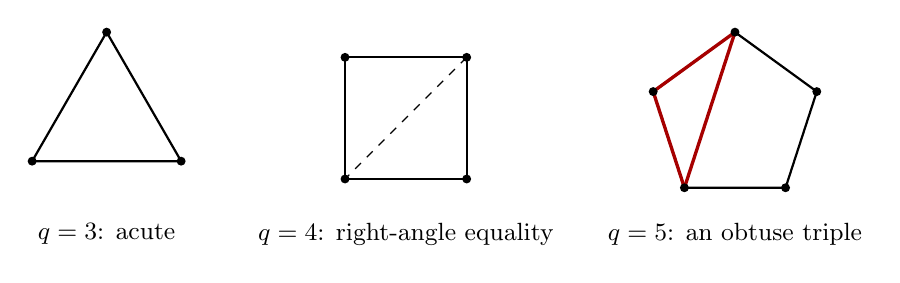
\begin{tikzpicture}[scale=0.95, every node/.style={font=\small}]
  % triangle
  \begin{scope}[xshift=0cm]
    \foreach \j in {0,1,2}{\coordinate (t\j) at ({90+120*\j}:1.15);}
    \draw[thick] (t0)--(t1)--(t2)--cycle;
    \foreach \j in {0,1,2}{\fill (t\j) circle (1.7pt);}
    \node at (0,-1.55) {$q=3$: acute};
  \end{scope}
  % square
  \begin{scope}[xshift=4cm]
    \foreach \j in {0,1,2,3}{\coordinate (s\j) at ({45+90*\j}:1.15);}
    \draw[thick] (s0)--(s1)--(s2)--(s3)--cycle;
    \draw[dashed] (s0)--(s2);
    \foreach \j in {0,1,2,3}{\fill (s\j) circle (1.7pt);}
    \node at (0,-1.55) {$q=4$: right-angle equality};
  \end{scope}
  % pentagon
  \begin{scope}[xshift=8.4cm]
    \foreach \j in {0,1,2,3,4}{\coordinate (p\j) at ({90+72*\j}:1.15);}
    \draw[thick] (p0)--(p1)--(p2)--(p3)--(p4)--cycle;
    \draw[very thick, red!65!black] (p0)--(p1)--(p2);
    \draw[very thick, red!65!black] (p0)--(p2);
    \foreach \j in {0,1,2,3,4}{\fill (p\j) circle (1.7pt);}
    \node at (0,-1.55) {$q=5$: an obtuse triple};
  \end{scope}
\end{tikzpicture}
\caption{The geometric threshold behind exactness. On a regular triangle or square, squared chordal distances satisfy the triangle inequalities. Starting with the pentagon, three consecutive vertices violate the squared-distance triangle inequality.}
\label{fig:polygon-cutoff}
\end{figure}


The image of the character $\chi$ is a regular $q(\chi)$-gon. The metric is squared Euclidean by construction and satisfies the triangle inequalities by Lemma \ref{lem:polygon-cutoff}. This gives us the following immediate corollary: 

\begin{corollary}\label{cor:low-q-feasible}
If $q(\chi)\leq 4$, then $d_\chi$ is feasible for GL.
\end{corollary}


The threshold also gives a particularly nice group characterization.

\begin{proposition}
\label{prop:universal-character-feasibility}
Each character metric on $\Gamma$ is feasible for GL if and only if $\exp(\Gamma)\leq 4$.
\end{proposition}

\begin{proof}
If $\exp(\Gamma)\leq 4$ then we have that each character image size divides the exponent and is at most four and so Corollary \ref{cor:low-q-feasible} applies. 
%explain this a bit better
For the opposite direction we note that if $\exp(\Gamma) = m\geq 5$ then the invariant-factor decomposition gives a character with image size $m$. Its regular-polygon metric violates a triangle inequality by Lemma \ref{lem:polygon-cutoff}.
\end{proof}





\subsection{Lossless rounding for images of size two, three, and four}
%Now we turn our attention to extracting the actual cut in the favorable cases of image sizes without any extra loss.  Explain that we start with the following result which shows that when the cyclic quotient induced by a character has at most four points then the spectral cost of that character can be converted to an explicit cut without any loss as the character kernel is optimal for quotients of order two or three while an order four quotient may require choosing between the two half-circle cuts but that is enough. This is the basic mechanism behind the exactness result for groups of exponent at most four. %explain in words what it does,
We now show that for $q \leq 4$ the character metric can also be rounded without loss:

\begin{lemma}
\label{lem:low-order-rounding}
Let $\chi\neq \mathbf{1}$ and let $q=q(\chi)\leq4$. Then $  \roundval(\chi)\le\lambda_\chi(G)$.
In particular (i) if $q=2$ or $q=3$ then $\psi_G(\ker\chi)=\lambda_\chi(G)$ and (ii) if $q=4$ then the best of the two half-circle quotient cuts has sparsity at most $\lambda_\chi(G)$.
\end{lemma}

\begin{proof}
Let $\beta=\Prb_{s\sim S}[\chi(s)\neq 1]$. If $q=2$ the only non-trivial phase is the $-1$. Each step with $\chi(s)\neq 1$ crosses the kernel and every step with $\chi(s)=1$ stays inside a kernel coset. Since $\mu(\ker\chi)=1/2$ we have $N_G(\ker\chi)=\beta$,  and $D(\ker\chi)=\nicefrac{1}{2}$, so $\psi_G(\ker\chi)=2\beta$. Also $\lambda_\chi(G)=1-[(1-\beta)\cdot1+\beta\cdot(-1)]=2\beta$.

If $q=3$, every nontrivial phase has real part $-1/2$. A nonkernel step translates the quotient by a nonzero residue. It crosses the singleton kernel exactly when its starting or ending phase is $0$, two disjoint events of probability $1/3$. Hence $N_G(\ker\chi)=\nicefrac{2}{3} \cdot \beta$,  $  D(\ker\chi)=2\cdot\frac{1}{3}\cdot\frac{2}{3}=\frac{4}{9}$ and $\psi_G(\ker\chi)=\frac{3}{2}\beta$.  The eigenvalue is the same: $\lambda_\chi(G)
  =1-[(1-\beta)\cdot1+\beta\cdot(-1/2)]
  =\nicefrac{3}{2}\beta$ .

%double check the explanation of double half circle cuts
Finally suppose $q=4$. We may label the phases $0,1,2,3$ around the square and we let $B_0=\{0,1\},   B_1=\{1,2\}$ and define $A_i=\chi^{-1}(B_i)$, then we get that on the square equal phases are separated by neither cut, adjacent phases are separated by exactly one cut, and finally opposite phases are separated by both which tells us that pointwise on $\Gamma\times\Gamma$ we have that $d_\chi=2d_{A_0}+2d_{A_1}$. Both of these cuts have density $\nicefrac{1}{2}$ and so $D(d_{A_0})=D(d_{A_1})=\nicefrac{1}{2}$. Using the Lemma \ref{lem:character-metric-ratio}
\[
  \lambda_\chi(G)
  ~=~ \frac{N_G(d_\chi)}{D(d_\chi)}
  ~=~ N_G(d_{A_0})+N_G(d_{A_1})
  ~=~ \frac{\psi_G(A_0)+\psi_G(A_1)}{2}
\]
and at least one of the two cuts has sparsity at most $\lambda_\chi(G)$.
\end{proof}

%\subsection{Exactness}
\begin{theorem}\label{thm:low-order-bottom-character}
Let $G=\Cay(\Gamma,S)$. Suppose there exists a nontrivial character $\chi$ such that $\lambda_\chi(G)=\lambda_2(G)$ and $q(\chi)\leq 4$.
Then
\[
  \lambda_2(G) ~=~ \gl(G) ~=~ \psi(G).
\]
Moreover, the optimal cut is explicitly obtained from $\chi$ as in Lemma \ref{lem:low-order-rounding}.
\end{theorem}

\begin{proof}
Using Corollary \ref{cor:low-q-feasible} and Lemma \ref{lem:character-metric-ratio} we have that $d_\chi$ is a feasible metric of objective value $\lambda_\chi(G)=\lambda_2(G)$ i.e., 
$\gl(G)\leq\lambda_2(G)$.  
Together with the spectral lower bound this gives us $\gl(G)=\lambda_2(G)$. By Lemma \ref{lem:low-order-rounding} we get that a quotient cut has sparsity at most $\lambda_\chi(G)=\lambda_2(G)$ and  combining with \eqref{eq:fundamental-chain} forces equality everywhere.
\end{proof}

\begin{corollary}[Exactness for exponent at most four]\label{cor:exp-four-exactness}
If $\exp(\Gamma)\leq 4$, then every Cayley graph $G=\Cay(\Gamma,S)$ satisfies $\lambda_2(G)=\gl(G)=\psi(G)$.
\end{corollary}

\begin{proof}
By equation \eqref{eq:lambda2-character-min} there is some nontrivial character which attains $\lambda_2(G)$ the image size of which divides $\exp(\Gamma)$ and is therefore at most four. Then we just apply Theorem \ref{thm:low-order-bottom-character}.
\end{proof}

%\begin{remark}
%The group exponent is a sufficient  condition and graph over a high exponent group is still exact when one of its bottom characters happens to have image size of at most four. 
%The theorem is spectral and dependent on the graph itself .
%Corollary \ref{cor:exp-four-exactness} is its  consequence when we extend to groups orders.
%\end{remark}

%Explain Why kernels are not enough at order four!
We finally note that kernels are not necessarily exact at order four with a simple example. Let $G=C_4=\Cay(\Z_4,\{1,-1\})$ and $\chi(x)=i^x$. The kernel is the singleton $\{0\}$. Four of the eight directed transitions cross it, so $N_G(\{0\})=\nicefrac{1}{2}$. Its denominator is $2 \cdot (1/4) \cdot (3/4)=\nicefrac{3}{8}$ giving $\psi_G(\ker\chi)=\nicefrac{4}{3}$.
But $\lambda_2(C_4)=1$, and the half-circle cut $\{0,1\}$ has numerator and denominator that are both $\nicefrac{1}{2}$ and so the quotient rounding is genuinely stronger than kernel rounding even in the smallest nontrivial case.
%\end{example}

%\subsection{Average distance in a cyclic direction}
%\subsection{The fully cyclically averaged graph}
%\subsection{Comparing metric objectives}
%\subsection{The Fourier spectrum after cyclic averaging}
%\subsection{From a bottom character to a cut}
%\subsection{The general approximation theorem}
%\subsection{Algorithmic form and consequences}



\section{Cyclic averaging and approximation}\label{sec:averaging}
When $q(\chi)\geq 5$, the squared chordal distance associated with $\chi$ violates the triangle inequality. This does not imply an integrality gap, since another feasible metric may still attain the cut optimum. In order to treat arbitrary character orders we will keep the GL feasible region unchanged but we will replace $G$ by a cyclically averaged walk in the same spirit as in \cite{dorsiaetall25}. In the next two subsections we will compare the metric objective values on $G$ and the cyclically averaged $G^\sharp$, and then compute the simplified Fourier spectrum of $G^\sharp$. We will then round a minimizing character by a cut in its cyclic quotient.


%Say that our goal is to obtain a guarantee for arbitrary finite Abelian Cayley graphs and thus we will take a different approach.  We have to leave the class of the feasible GL metrics unchanged and instead say that we  introduce an auxiliary random walk. Say where this walk comes from. For each generator $s$ we will replace the single move s by a uniformly random multiple of s inside the complete cyrclic subgroup generated by s (including the zero multiple). This will achieve two **complementary goals**: first, an auxiliary move by \ell times s can be simulated by a shortest sequence of the original moves plus or minus s.  The triangle inequalities therefore compare the objective of every feasible metric on the auxiliary graph withits objective on the original primal graph and then the loss then is the average cyrclic distance needed to simulate a uniformly random multiple of s

%Second, I notice that performing a full subgroup averaging greatly simplifies the Fourier spectrum: Let me explain, if we are given a character chi then the exact position of chi(s) on the unit circle is of no importance.  The averaged spectral contribution of s is zero when moving by s leaves the character unchanged, and one otherwise. As a result we get that, roughly speaking, a character has a small eigenvalue exactly when it is constant along most generator directions.  Most such generators lie inside kernel of \chi so that the this kernel provides a very natural choice for sparse cut!

\iffalse
The proof of the general theorem therefore has three stages:
\[
  \boxed{
  \begin{array}{c}
  \text{compare metric objectives under cyclic averaging}\\
  \Downarrow\\
  \text{compute the simplified character spectrum}\\
  \Downarrow\\
  \text{convert a bottom auxiliary character into a cut}.
  \end{array}}
\]
We carry out these stages in order.
\fi

\subsection{Metric objectives under full cyclic averaging}
Let $r\geq 2$ and $0 \leq \ell \leq r-1$ (note that we include the 0 to be fully cyclic), then define
\begin{equation}\label{eq:Lr-def}
  L_r(\ell)=\min\{\ell,r-\ell\}.
\end{equation}
to be the smallest number of $+/-1$ steps from $0$ to $\ell$ in the cycle $\Z_r$. We also define
\begin{equation}\label{eq:alpha-def}
  \alpha(r)~=~\frac1{r}\sum_{\ell=0}^{r-1}L_r(\ell) 
  ~=~ \begin{cases}
    \nicefrac{r}{4},&r\text{ even},\\[6pt]
    \frac{r^2-1}{4r},&r\text{ odd}
  \end{cases}.
\end{equation}
to be the average distance around a cycle of length $r$ and it measures how much we have to pay if we replace one generator step by a uniformly random move in the cyclic subgroup it generates. For the closed form of $\alpha(r)$ we notice that for $r=2k$ then 
\[
  \sum_{\ell=0}^{r-1}L_r(\ell)
  =2(1+\cdots+(k-1))+k=k^2,
\]
so $\alpha(2k)=k^2/(2k)=k/2=r/4$.
If $r=2k+1$
\[
  \sum_{\ell=0}^{r-1}L_r(\ell)
  =2(1 + \cdots + k)=k(k+1),
\]
so $\alpha(2k+1)=k(k+1)/(2k+1)=\nicefrac{(r^2-1)}{4r}$. 
Moreover, $\alpha(r)$ is nondecreasing and $\alpha(r)=r/4+\mathcal{O}(1)$. 
%Indeed 
%\[
%\alpha(2k)=\frac{k}{2} \leq \frac{k(k+1)}{2k+1}=\alpha(2k+1) \leq \nicefrac{k+1}{2} = \alpha(2k+2)
%\]

For the generator multiset $S$ we subsequently define
\begin{equation}\label{eq:rho-def}
  \rho(S)=\max_{s\in S}\alpha(\ord(s))
\end{equation}
which is the worst such cost among all the generators which is precisely the loss we will suffer when we wish to compare GL metrics before and after the cyclic averaging.

We now construct the fully cyclically averaged  graph:
\begin{definition}[Cyclic averaging]\label{def:cyclic-averaging}
%For each occurrence $s\in S$ 
The cyclically averaged walk $G^\sharp$ is the symmetric weighted Abelian Cayley random walk generated with the following steps:
\begin{enumerate}
  \item we sample an occurrence $s\sim S$ and $\ell$ uniformly from $\{0,\ldots,r_s-1\}$, then
  \item move from $x$ to $x+\ell s$.
\end{enumerate}
\end{definition}

%Equivalently, since all transition weights are rational we can realize $G^\sharp$ as a regular Cayley multigraph with the same normalized random walk operator. The distribution is symmetric because $\ell s$ and $(r_s-\ell)s=-\ell s$ have the same conditional probability. 
%Repeated original generators remain repeated.  If two different generators generate the same cyclic subgroup, their contributions are also remains separately.

We note that the inclusion of the zero element turns cyclic averaging into an exact subgroup projection but, on the other hand, the exclusion of it it leaves a shifted  version of that projection that depends on the order.


\subsection{Averaged path inequality}
In order to compare $G^\sharp$ with $G$ we will represent each averaged step $\ell \cdot s$ with a shortest path of $L_{r_s}(\ell)$ steps in the directions $+s$ or $-s$ and we will then average the resulting triangle inequality over the starting vertex.
%When we defined the cyclically averaged graph G^\sharp explain that its main property was that its Fourier spectrum is much simpler than the one of the primal graph G. However, by itself yhis simplification of the Fourier spectrum of G^\sharp is not enough as we would like to compare the metric objective on G^\sharp with the metric objective on the original graph. If we fix a  metric d, then these numerators are N_G(d)=\mathbb E_{s,x}d(x,x+s) and N_{G^\sharp}(d) =\mathbb E_{s,\ell,x}d(x,x+\ell s) respectively. What we do need is to be able to somehow control the average cost of the cyclic steps \ell s in terms of the cost of the original step s.

%It is actually tempting to consider that for the pointwise estimate
%\[
%    d(x,x+\ell s)
%      \leq L_{r_s}(\ell)\,d(x,x+s),
%\]
%but this is unfortunately not true because the triangle inequality splits the long step into short edges having different starting points. A small example: for the cut metric associated with $A=\{0,1\}\subseteq\mathbb Z_4$ we have that $d_A(0,2)=1$ but $d_A(0,1)=0$ and so even the simple inequality $d_A(0,2)\leq2d_A(0,1)$ fails.

%The pointwise estimate is stronger than what we need. 
\iffalse
Note that the graph numerator already averages uniformly over the starting vertex $x$ and after this averaging each translated short edge
$(x+js,x+(j+1)s)$ has the same expected length as $(x,x+s)$ and 
as a consequence, the triangle inequality gives us
\[
    \mathbb E_x d(x,x+\ell s)
      ~\leq~
    L_{r_s}(\ell)\,\mathbb E_x d(x,x+s).
\]
If we average this inequality over $\ell$ and over $s$ will give us $N_{G^\sharp}(d)\leq \rho(S)N_G(d)$, which is exactly what we need to compare the GL between the primal $G$ and $G^\sharp$. 
\fi

%We formalize this idea below. 

%The triangle inequalities ``decomposes'' a long cyclic step as a sum of short individual steps but they do \emph{not} control it pointwise by a multiple of the particular short edge starting at the same vertex. For example, in the cut metric of $A=\{0,1\}\subset\Z_4$ we have that $d_A(0,2)=1$ but $d_A(0,1)=0$ i.e., the longer step from $0$ to $2$ crosses the cut even though the short step from $0$ to $1$ does not. If we average over the starting point removes this 
% When we replace s by a random multiple \ell s we wish to be able to bound $\E_x d(x,x+\ell s)$ but using the original $s$-direction cost $\E_x d(x,x+s)$  this is what we do in the following lemma with $L_r(\ell)$ to be equal to the number of original plus/minus s-steps we need in order to simulate \ell s. Averaging subsequently over \ell gives us exactly \alpha(r) and then averaging over s gives \rho(S)

\begin{lemma}[Averaged cyclic path inequality]\label{lem:averaged-path}
Let $d$ be a metric on $\Gamma$. For each nonzero $s\in\Gamma$ with $r=\ord(s)$ and each $1\leq \ell \leq r-1$ we have that
\begin{equation}\label{eq:averaged-path}
  \E_{x\sim\Gamma}d(x,x+\ell s)
  ~\leq~ L_r(\ell) \cdot \E_{x\sim\Gamma}d(x,x+s).
\end{equation}
\end{lemma}

\begin{proof}
Let $L=L_r(\ell)$. In the cyclic subgroup $\langle s\rangle$ we choose a shortest path $0=y_0,y_1,\ldots,y_L=\ell s$ the increments of which are all either $+s$ or all $-s$. Now for each $x$ the triangle inequality gives us
\[
  d(x,x+\ell s)
  ~\leq~ \sum_{j=0}^{L-1}d(x+y_j,x+y_{j+1}).
\]
We now average over uniform $x$. If $y_{j+1}-y_j=s$, translation invariance gives
\[
  \E_x d(x+y_j,x+y_j+s)=\E_u d(u,u+s).
\]
If the step is $-s$ then symmetry of $d$ and a change of variables give
\[
  \E_xd(x+y_j,x+y_j-s)=\E_ud(u,u-s)=\E_ud(u,u+s).
\]
Each one of the $L$ terms has the same average and this the claim.
\end{proof}

\begin{proposition}\label{prop:metric-averaging}
For each metric $d$ on $\Gamma$,  $N_{G^\sharp}(d)  ~\leq~ \rho(S) \cdot N_G(d)$
%\begin{equation}\label{eq:averaging-N}
%  N_{G^\sharp}(d)  ~\leq~ \rho(S) \cdot N_G(d).
%\end{equation}
and, consequently, $\gl(G^\sharp) \leq \rho(S) \cdot \gl(G)$.
%\begin{equation}\label{eq:averaging-arv}
%  \gl(G^\sharp) ~\leq~ \rho(S) \cdot \gl(G).
%\end{equation}
\end{proposition}

\begin{proof}
Let us fix an occurrence $s\in S$. The Averaging Lemma \ref{lem:averaged-path} over uniform $\ell \in\{0,\ldots,r_s-1\}$ gives
\[
  \frac{1}{r_s}\sum_{\ell=0}^{r_s-1}
  \E_xd(x,x+\ell s)
  \leq \alpha(r_s)\E_xd(x,x+s).
\]
We note that the $\ell = 0$ term is zero and we average over $s\sim S$ and use $\alpha(r_s)\le\rho(S)$, the first inequality of the statement.

For a feasible GL metric, the denominator $D(d)=\E_{x,y}d(x,y)$ depends only on the uniform vertex measure, not on the graph. Therefore
\[
  \frac{N_{G^\sharp}(d)}{D(d)}
  ~\leq~ \rho(S) \cdot \frac{N_G(d)}{D(d)}.
\]
Finally, it is enough to take the infimum over the feasible metrics for $G$.
\end{proof}



%\begin{remark}[Relation to walk powers]
We remark that  Oveis Gharan  and Trevisan compare a GL solution on $G$ with the same solution on a walk-power graph $G^t$, controlling the increase by decomposing a random long walk and averaging over translations \cite{Trevisan21}. In our Proposition \ref{prop:metric-averaging} above we use the same  averaging idea but on a different graph: \emph{averaging} treats each cyclic generator direction independently which means that the loss depends on the cyclic order and neither on the random-walk length nor on the actual degree.
%\end{remark}

%The averaging comparison is purely metric. Its usefulness comes from the unusually simple Fourier spectrum of $G^\sharp$.


\subsection{The simplified Fourier spectrum}
%The following Lemma gives us the simplified Fourier spectrum after we have performed the cyclic averaging:
%Full cyclic averaging gives the following exact kernel-indicator formula for the Fourier spectrum.
The Fourier spectrum of the cyclically averaged walk has the following simplified and useful form:
%that  performing full cyclic averaging removes both the phase and the generator order from the character contribution as a generator contributes exactly 0 if it lies in $\ker \chi$, and exactly 1 otherwise. 

\begin{lemma}[Spectrum of $G^\sharp$]\label{lem:saturated-spectrum}
For each character $\chi\in\Gammahat$ we have
\begin{equation}\label{eq:saturated-spectrum}
  \lambda_\chi(G^\sharp)
  =\E_{s\sim S} ~\one_{\{\chi(s)\neq 1\}}.
\end{equation}
\end{lemma}

\begin{proof}
We fix an occurrence $s \in S$ and recall that $r_s = \ord(s)$. Then the conditional adjacency contribution is 
\[
\frac{1}{r_s} \sum_{\ell=0}^{r_s-1} \chi(\ell s) 
~=~
\frac{1}{r_s} \sum_{\ell = 0}^{r_s-1} \chi(s)^\ell.
\]
If $\chi(s) = 1$ then this average equals to one so the conditional Laplacian contribution is  zero otherwise the $\chi(s)$ is a non-trivial root of unity the order of which divides the order $r_s$ and the summation above becomes zero.  We average over $s \sim S$ and conclude the statement of the Lemma.

\iffalse
Fix an occurrence $s\in S$. Its conditional adjacency contribution is
\[
  \frac1{r_s-1}\sum_{\ell=1}^{r_s-1}\chi(\ell s).
\]
If $\chi(s)=1$, this average equals $1$, so the Laplacian contribution is zero. Suppose $\chi(s)\ne1$. The value $z=\chi(s)$ is a nontrivial root of unity whose order divides $r_s$. Hence
\[
  \sum_{\ell=0}^{r_s-1}z^\ell=0 \mbox{ and thus }  \sum_{\ell=1}^{r_s-1}z^\ell=-1.
\]
The adjacency contribution is therefore $-1/(r_s-1)$ and the Laplacian contribution is $1+\frac1{r_s-1}=\frac{r_s}{r_s-1}$.
A simple average over $s\sim S$ concludes the result.
\fi
\end{proof}

%In words, blah blah blah



\subsection{Kernel rounding and the approximation}
%The formula above has a nice combinatorial meaning. 
%A character has small auxiliary eigenvalue exactly when it is unchanged along most of the generator directions. 
The directions under which a character remains unchanged lie in its kernel and they preserve every kernel coset. We can calculate the contribution to the kernel cut of the remaining directions. In the following we assume $\chi\ne\mathbf{1}$, let $q=q(\chi)$.
%how the remaining directions exactly contribute to  the kernel cut

\begin{lemma}[Kernel rounding with image-size factor]\label{lem:kernel-rounding}
We have that
\begin{equation}\label{eq:kernel-beta}
  \psi_G(\ker \chi)
  ~=~ \frac{q}{q-1} \cdot \Prb_{s\sim S}[\chi(s)\neq 1]
  ~=~ \frac{q}{q-1} \cdot \bigg[\lambda_\chi(G^\sharp)\bigg].
\end{equation}
%and
%\begin{equation}\label{eq:kernel-vs-saturated-eigenvalue}
%  \psi_G( \ker \chi)
%  ~=~ \frac{q}{q-1} \cdot \bigg[\lambda_\chi(G^\sharp)\bigg].
%\end{equation}
\end{lemma}

\begin{proof}
We first set $\beta=\Prb_{s\sim S}[\chi(s)\neq 1]$.
By \eqref{eq:kernel-density} the $\mu(K)$ is equal to $1/q$. If $\chi(s)=1$ translation by $s$ preserves every kernel coset and never crosses $K = \ker \chi$. If $\chi(s)\ne1$ then of course $K$ and $K-s$ are disjoint. A directed edge $(x,x+s)$ crosses $K$ when either $x\in K$ or $x\in K-s$ and so the  probability of crossing (over some  $x$) is $2/q$ and so we can conclude that $N_G(K)=\nicefrac{2\beta}{q}$.
The denominator on the other hand is $D(K) = 2 \cdot \nicefrac{1}{q} \cdot \left(1-\nicefrac{1}{q}\right) = \frac{2(q-1)}{q^2}$.
Dividing the two terms gives us \eqref{eq:kernel-beta}. By the previous Lemma \ref{lem:saturated-spectrum} we have that $\lambda_\chi(G^\sharp) = \Pr_s[\chi_s \neq 1]$ so we get the claimed equality.
%Finally, each nonzero contribution in \eqref{eq:saturated-spectrum} has weight $r_s/(r_s-1)\geq 1$  i.e., $\lambda_\chi(G^\sharp)\geq\beta$.
\end{proof}

%\subsection{The general theorem}
%We are now in a position to assemble everything and to give the general Rounding Theorem:
The combination of Corollary \ref{cor:quotient-kernel-chain} and Lemma \ref{lem:kernel-rounding} give 
\[
  \psi(G)
  ~\leq~\roundval(\chi^*)
  ~\leq~\psi_G(\ker\chi^*)
  ~=~\frac{q^*}{q^*-1}\cdot \bigg[\lambda_{\chi^*}(G^\sharp)\bigg].
\]
Since the quantity $\chi^*$ minimizes among the nontrivial characters we have that $\lambda_{\chi^*}(G^\sharp)=\lambda_2(G^\sharp)$. 
On the other hand, by the spectral lower bound and the averaging comparison we get
\[
  \lambda_2(G^\sharp)
  ~\leq~\gl(G^\sharp)
  ~\leq~\rho(S) \cdot \gl(G).
\]
Combining the above and using that $q^*/(q^*-1)\leq2$ we get the main approximation theorem: 
%gives \eqref{eq:general-round-bound}. Since $q^*/(q^*-1)\le2$, \eqref{eq:two-rho} follows.
\begin{theorem}[Cyclic averaging and quotient rounding]\label{thm:general-bound}
Let $G=\Cay(\Gamma,S)$ and let $\chi^*$ be a nontrivial character minimizing $\lambda_\chi(G^\sharp)$ i.e., $\chi^* \in \arg \min \Pr_s[\chi(s) \neq 1]$. Set $q^*=q(\chi^*)=|\chi^*(\Gamma)|$.
Then
\begin{equation}\label{eq:general-round-bound}
  \psi(G)
  ~\leq~ \roundval(\chi^*)
  ~\leq~ \frac{q^*}{q^*-1}\rho(S)\gl(G).
\end{equation}
%In particular,
%\begin{equation}\label{eq:two-rho}
%  \psi(G) ~\le~ 2\rho(S) \cdot \gl(G).
%\end{equation}
The explicit kernel cut $K=\ker\chi^*$ satisfies the same right-hand side in \eqref{eq:general-round-bound}.
\end{theorem}



\begin{corollary}\label{cor:bounded-order}
For connected $G$, if each generator has order at most $R$ then
\[
  \frac{\psi(G)}{\gl(G)}\leq 2 \cdot \alpha(R)
  =
  \begin{cases}
    \nicefrac{R}{2},&R\text{ even}, \\
    \nicefrac{R^2-1}{2R},&R\text{ odd}.
  \end{cases}
\]
%In particular, the gap is at most $R/2+\mathcal O (1)$.
\end{corollary}

%\begin{proof}
%\end{proof}

\subsection{Algorithm}

The proof also yields an explicit algorithm that does not solve the SDP.


\begin{corollary}[Explicit kernel algorithm]\label{cor:kernel-algorithm}
Assume the finite Abelian group is given by an explicit cyclic decomposition and the symmetric generator multiset $S$ is given explicitly. In time polynomial in $n=|\Gamma|$, $|S|$, and the bit length of the decomposition, one can output a cut $K$ satisfying
%\[
%  \psi_G(K) ~\leq~ 2\rho(S)\psi(G).
%\]
%More precisely, the algorithm outputs $K=\ker\chi^*$ and satisfies
\[
  \psi_G(K)
  ~\leq~ \frac{q^*}{q^*-1} \cdot \rho(S) \cdot \gl(G).
\]
\end{corollary}

\begin{proof}
The explicit decomposition lists all $n$ characters as product characters. For each nontrivial $\chi$ we compute \eqref{eq:saturated-spectrum} exactly. This is easy as it only requires for testing whether $\chi(s)=1$ and for knowing the $\ord(s)$. Choose a minimizer $\chi^*$ and output its kernel. The value guarantee follows by Theorem \ref{thm:general-bound} and by using $\gl(G) \leq \psi(G)$.
%we xompute the corresponding approximation ratio.
\end{proof}

\begin{remark}
%Input model, maybe move in the beiginning?
Enumerating all $|\Gamma|$ characters is polynomial in $n=|\Gamma|$. It can be exponential in a succinct description whose bit length is only $\mathcal{O}(\log|\Gamma|)$. The algorithmic claim is made in the explicit $n$-vertex/group decomposition model.
\end{remark}


%Given $\chi$ with image size $q$, we can compute the exact value $\roundval(\chi)$  by checking all the cuts of the $q$-vertex quotient, in time $2^{q-1}\poly(q,|S|)$. This can may improve the kernel substantially, but I do not think we need it for the polynomial-time $2\rho(S)$ guarantee.


Finally, we parallel Lemma 8.2 from d'Orsi et al. \cite{dorsiaetall25} for Cayley graphs over $\mathbb{F}_p^k$, $p$ prime. 


\begin{corollary}\label{cor:prime-exponent}
Let $p$ be prime and let $G=\Cay(\mathbb{F}_p^k,S)$ be connected. If $p\ge5$, then
\begin{equation}\label{eq:prime-bound}
  \frac{\psi(G)}{\gl(G)}
  ~\leq~\frac{p}{p-1} \cdot \alpha(p) 
  = \frac{p}{p-1} \cdot \frac{(p-1)(p+1)}{4p} 
  ~=~ \frac{p+1}{4}.
\end{equation}
%For $p=5$, the bound is $15/8$. For $p=2$ or $3$ Corollary \ref{cor:exp-four-exactness} gives the stronger value $1$.
\end{corollary}

\begin{proof}
Every nonzero generator has order $p$, so $\rho(S)=\alpha(p)$. Every nontrivial character of $\mathbb{F}_p^k$ has image size exactly $p$, so $q^*=p$. We apply Theorem \ref{thm:general-bound} and use $\frac{p}{p-1} \alpha(p)=\frac{p+1}{4}$ for odd $p$.
\end{proof}

\begin{remark}
In this prime field setting, our metric comparison is an SDP extension of d’Orsi et al. Lemma 8.2  for the comparison for cut metrics. They prove a  $\nicefrac{p+1}{4}$ bound but in our case this holds more generally \emph{for each Goemans–Linial feasible metric} instead of only cut metrics as in d'Orsi et al. When we combine our bound with the exact kernel identity  we are able to prove the integrality gap bound $\psi(G)/\gl(G) \leq \nicefrac{p+1}{4}$ (something that does not, at least not directly, follow from d'Orsi et al.). 
%Our  contribution remains Theorem \ref{thm:general-bound} which is applied on arbitrary finite Abelian groups even with mixed generator orders. In that setting there is no single prime $p$, the nonzero-multiple spectrum acquires order-dependent factors, and including zero gives us the useful simpler eigenspectrum of the coefficients. But should be clear so far
\end{remark}



%\section{Sharpness of the individual constants}

%TWe show that the metric averaging factor $\alpha(r)$ is exact. It is important to note that these statements are about the individual inequality and not about the optimal quotient value or the full gap

\subsection{Exact averaging constant}
The two constants in Theorem \ref{thm:general-bound} arise from different steps. We show that the metric averaging factor $\alpha(r)$ is exact. 


\begin{theorem}\label{thm:alpha-optimal}
For every $r\ge2$,
\begin{equation}\label{eq:alpha-optimal}
  \sup_d
  \frac{
    \frac1{r}\sum_{\ell=0}^{r-1}\E_{x\in\Z_r}d(x,x+\ell)
  }{
    \E_{x\in\Z_r}d(x,x+1)
  }
  =\alpha(r),
\end{equation}
where the supremum is over all metrics $d$ with positive denominator. The supremum is attained by a cut metric and hence also within the GL-feasible class.
\end{theorem}

\begin{proof}
The upper bound is Lemma \ref{lem:averaged-path} averaged over $\ell$. For the lower bound, let $m=\lfloor r/2\rfloor$ and take the interval $A=\{0,1,\ldots,m-1\}\subset\Z_r$. We use its cut metric $d_A$. For a shift $\ell$ the symmetric difference of the interval and its translation has size $|A\triangle(A-\ell)|~=~2L_r(\ell)$.

This is easy to see once we choose the shorter orientation around the cycle. If we shift an interval by $L_r(\ell)$ we remove exactly $L_r(\ell)$ points at one boundary but at the same time we add the same number at the other. In the even antipodal case the two intervals are complementary and the same formula gives $r$. Therefore
\[
  \E_xd_A(x,x+\ell)=\frac{2L_r(\ell)}r,
  \qquad
  \E_xd_A(x,x+1)=\frac2r.
\]
The ratio in \eqref{eq:alpha-optimal} is exactly $  \frac1{r}\sum_{\ell=0}^{r-1}L_r(\ell)=\alpha(r)$.
\end{proof}


\iffalse
\subsection{Sharpness of kernel rounding}

\begin{proposition}[Optimality of the kernel factor]\label{prop:kernel-sharp}
For every integer $q\ge2$ and every $\eps>0$, there exist an Abelian Cayley graph $G$, a character $\chi$ with $q(\chi)=q$, and $K=\ker\chi$ such that
\[
  \frac{\psi_G(K)}{\lambda_\chi(G^\sharp)}
  ~\geq~ \frac{q}{q-1}-\eps.
\]
\end{proposition}

\begin{proof}
let us fix $q$ and take $\Gamma=\Z_{qm}$ with $S=\{1,-1\}$ and define $\chi(x)=e^{2\pi ix/q}$ which has image size $q$. Its kernel is
\[
  K=\big\{x:x\equiv0\pmod q\big\},
\]
with density $1/q$. For each original step $+1$ or $-1$ the directed edge crosses $K$ exactly in the case when its starting or ending point happens to be a multiple of $q$ and this  event happens with probability $2/q$. Hence
\[
  N_G(K)=\frac2q,
  \quad
  D(K)=2\frac1q\left(1-\frac1q\right),
  \quad \mbox{and } \psi_G(K)=\frac{q}{q-1}.
\]

Since $1$ generates the $\Z_{qm}$, cyclic averaging makes the step uniform over every  group element, including the zero element. Thus $G^\sharp$ is the normalized complete Cayley graph on $qm$ vertices. Every nontrivial character has eigenvalue $\lambda_\chi(G^\sharp)=1$. As a consequence we have that
\[
  \frac{\psi_G(K)}{\lambda_\chi(G^\sharp)}
  ~=~\frac{q}{q-1}.
\]
\end{proof}
\fi


%Theorem \ref{thm:alpha-optimal} 
%together with Proposition \ref{prop:kernel-sharp} 
%together with the equality achieved already by the kernel rounding in  Lemma \ref{lem:kernel-rounding} shows us that the metric averaging comparison and the kernel rounding inequality are separately sharp however they do **not** show that the inequality \psi(G)\leq 2\rho(S)\gl(G) is tight. 
%In the example of Proposition {prop:kernel-sharp}, the best cut in the quotient may very well be much better than the singleton kernel and even more generally, the metric comparison, spectral lower bound, and rounding step may not necessarily be simultaneously tight on one graph.
%\end{remark}

\section{Some examples and some consequences}\label{sec:examples}

We  give some examples that illustrate both the strength and the limitations of the  bounds of the previous sections. In particular, we discuss how $\rho(S)$ may be far away from the actual Goemans–Linial gap. 

\subsection{Cubelike graphs and exponent three and four}
A cubelike graph is a Cayley graph over $\mathbb{F}_2^k$. By Corollary \ref{cor:exp-four-exactness} each cubelike graph satisfies $\lambda_2(G)= \gl(G)= \psi(G)$ and an optimal cut is a hyperplane, namely the kernel of a bottom character.

We note that the  exact spectral solvability is already observed by d’Orsi et al. \cite{dorsiaetall25}: the Boolean Fourier characters are $\{\nicefrac{+1}{-1}\}$ valued and a bottom character indicates an optimal cut but our results recover this and extends the same exactness to all finite Abelian groups of exponent three and four.

%At exponent three the kernel of a bottom character is optimal. At exponent four exactness still holds, but kernel rounding can fail as the $C_4$ example shows that a half-circle quotient cut may instead be required.


\subsection{Cycles}
%are exact despite large generator order

The  bound in Theorem \ref{thm:general-bound} is weak on a cycle because the generator has order $n$. On the positive side, the underlying averaging inequality is strong enough to determine the exact GL value.

\begin{proposition}
% the Exact GL value on cycles
\label{prop:cycle-exact}
For each $n\geq 3$,
\begin{equation}\label{eq:cycle-exact}
  \gl(C_n)=\psi(C_n)
  =
  \begin{cases}
    4/n,& n \text{ is even},\\[6pt]
    (4n)/(n^2-1),&n\text{ is odd}.
  \end{cases}
\end{equation}
In fact, the same value is obtained if the SDP is relaxed further to all metrics satisfying the triangle inequalities, without the squared-Euclidean requirement.
\end{proposition}

\begin{proof}
Let $d$ be any metric on $\Z_n$. Averaging the generator $1$ makes the random step uniform over $\Z_n$ so $C_n^\sharp=\Cay(\Z_n,\Z_n)$ in normalized random-walk form where the zero step is just a self loop. Since $d(x,x)=0$ we have that
\[
  N_{C_n^\sharp}(d)
  =\frac1{n^2}\sum_{x \neq y}d(x,y) ~=~ D(d).
\]
By Proposition \ref{prop:metric-averaging} we have $D(d) \leq \alpha(n) \cdot N_{C_n}(d)$ and so every metric satisfies
\begin{equation}\label{eq:cycle-metric-lower}
  \frac{N_{C_n}(d)}{D(d)}
  ~\geq~\frac{1}{\alpha(n)}.
\end{equation}

Now let $m=\lfloor n/2\rfloor$ and take the interval cut $A=\{0,1,\ldots,m-1\}$. Exactly two undirected cycle edges cross the cut, equivalently four of the $2n$ directed transitions cross, so $N_{C_n}(A)=\nicefrac{2}{n}$. Its denominator is $D(A) = 2 \cdot \frac{m}{n} \left(1-\frac{m}{n}\right) = \frac{2m(n-m)}{n^2}$.
Therefore
\[
  \psi_{C_n}(A)=\frac{n}{m(n-m)}
  =
  \begin{cases}
    4/n,&n\text{ even},\\[3pt]
    4n/(n^2-1),&n\text{ odd}.
  \end{cases}
\]
Using the closed form for $\alpha$ the lower bound in \eqref{eq:cycle-metric-lower} is exactly the same quantity. Hence the metric relaxation, the GL relaxation, and the cut optimum all coincide.
\end{proof}

\begin{remark}
\label{remark:gaps}
For cycles $\rho(\{\nicefrac{-1}{+1}\})=\alpha(n)=\Theta(n)$ and $\frac{\psi(C_n)}{\gl(C_n)}=1$. Thus $\rho(S)$ can overestimate the true GL gap by a linear factor. At the same time $\lambda_2(C_n)=1-\cos(2\pi/n)=\Theta(n^{-2})$ but $\gl(C_n)=\Theta(n^{-1})$ from which we get that
\[
  \frac{\gl(C_n)}{\lambda_2(C_n)}=\Theta(n).
\]
\end{remark}



\subsection{Discrete tori}\label{subsec:tori}

Fix $r\ge5$ and $k\ge1$, and consider the Cartesian power of a cycle $C_r^{\square k}
  =\Cay((\Z_r)^k,\{\pm e_1,\ldots,\pm e_k\})$ which we denote by $T_{r,k}$. 
This graph has degree $2k$ and each generator has order $r$. 

\begin{proposition}
\label{prop:torus}
Let $a=\lfloor r/2\rfloor$. Then
\begin{equation}\label{eq:torus-lambda}
  \lambda_2(T_{r,k}) ~=~ \frac{1-\cos(2\pi/r)}{k}
\end{equation}
and
\begin{equation}\label{eq:torus-cut}
  \psi(T_{r,k}) ~\leq~ \frac{r}{k \cdot a(r-a)}.
\end{equation}
As a result
\begin{equation}\label{eq:torus-gap}
  \frac{\psi(T_{r,k})}{\gl(T_{r,k})}
  ~\leq~
  \frac{r}{a(r-a)(1-\cos(2\pi/r))},
\end{equation}
a constant depending on $r$ but not on $k$. 
%For $r=5$,
%\[
%  \frac{\psi(T_{5,k})}{\gl(T_{5,k})}
%  ~\leq~ \frac{5+\sqrt5}{6} ~<~ 1.207.
%\]
\end{proposition}

\begin{proof}
For $t=(t_1,\ldots,t_k)\in(\Z_r)^k$, the character $\chi_t$ has Laplacian eigenvalue equal to $\lambda_t = 1-\frac{1}{k}\sum_{j=1}^k\cos(2\pi t_j/r)$.
For a nonzero $t$, at least one coordinate is nonzero, and the largest cosine at a nonzero residue is $\cos(2\pi/r)$. We get the minimum eigenvalue by taking one coordinate equal to plus/minus $1$ and all others zero, giving \eqref{eq:torus-lambda}.

Take the coordinate interval cut $A=\{x:x_1\in\{0,1,\ldots,a-1\}\}$. 
Only the two directions $+/- e_1$ can cross. Conditioning on choosing one of those directions, exactly two of the $r$ possible values of $x_1$ can cross the interval boundary so $N_{T_{r,k}}(A)=\frac1k\cdot\frac2r=\frac{2}{kr}$. The density is $a/r$ and so $D(A)=2\frac{a}{r} \left(1-\frac{a}{r} \right)=\frac{2a(r-a)}{r^2}$. Their ratio is \eqref{eq:torus-cut}. Finally, $\gl \geq  \lambda_2$ gives \eqref{eq:torus-gap}.

For $r=5$, $a=2$ and $1-\cos(2\pi/5)=(5-\sqrt5)/4$ which gives $\nicefrac{5}{6(1-\cos(2\pi/5))}=\nicefrac{(5+\sqrt5)}{6}$.
\end{proof}


%Mention that the bound in Proposition \{prop:torus} is stronger than the generic averaging certificate on this particular family and it uses only an explicit cut plus the spectral lower bound. Its  purpose is to  show that a fixed generator order can exist with unbounded degree and a uniformly small true gap in a natural family outside the exponent-four case which is exact.



\subsection{An  $\nicefrac{16}{15}$ integrality gap family}\label{subsec:integrality}
We next give an explicit connected Abelian Cayley graph on which the Goemans–Linial relaxation is not exact, and then extend it to an infinite family. To the best of our knowledge, no previously published explicit finite Abelian Cayley graph with uniform demands has been shown to have Goemans–Linial gap strictly larger than one. The seed graph has ten vertices and gap $16/15$. 


We begin with the initial seed graph. Let $C=\operatorname{Cay}\bigl(\mathbb Z_{10},\{\pm1,\pm3\}\bigr)$. Combinatorially, $C$ is $K_{5,5}$ with a perfect matching removed. Then we will show that 
$\lambda_2(C)=\operatorname{SDP_{GL}}(C)=\nicefrac{3}{4}$ and $\psi(C)=\nicefrac{4}{5}$ and so for this small graph we have 
\[
\frac{\psi(C)}{\operatorname{SDP_{GL}}(C)}=\frac{16}{15}.
\]


Indeed for $j\in\mathbb Z_{10}$  let $\chi_j(t)=e^{2\pi ijt/10}$. Proposition \ref{prop:character-diagonalization} about character diagonalization gives $1-\frac12\left( \cos\frac{\pi j}{5} + \cos\frac{3\pi j}{5} \right)$. The smallest nonzero eigenvalue is attained at $j\in \{1,3,7,9\}$, and equals to $\lambda_2(C)=\nicefrac{3}{4}$.

To obtain a matching GL solution we define the translation-invariant semimetric $d_0 = \nicefrac{1}{4}d_{\chi_1} + \nicefrac{1}{4}d_{\chi_3}$ given by the formula
\[
d_0(x,y) ~=~ \frac{1}{2}\left(1-\cos\frac{\pi(y-x)}5\right)
+
\frac{1}{2}\left(1-\cos\frac{3\pi(y-x)}5\right).
\]
This is squared Euclidean distance because it is a nonnegative combination of squared character distances. Its values depend only on $t=y-x$ and are 
\[
d_0(t)=
\begin{cases}
0, & t=0 \\
\nicefrac{3}{4}, & t\in \{ -3,-1,+1,+3 \} \\
\nicefrac{5}{4}, & t\in \{-4,-2,+2,+4\} \\
2, & t=5.
\end{cases}
\]
We first verify the triangle inequalities. If the longest side has length at most $5/4$ then (unless one of the other sides is zero) their sum is at least $\frac34+\frac34>\frac54$. We now  consider a triangle the longest side of which has length $2$, which corresponds to two points whose difference is $5$. In any decomposition $5=u+v$ with $u,v\neq 0$ one term of the sum must be  odd while the other must be even number and none can be $0$ or $5$ and therefore $d_0(u)+d_0(v) = \frac34+\frac54=2 = d_0(5)$. Thus $d_0$ is feasible for the GL relaxation. 


%$\frac1{10} \left( 4\cdot\frac34+4\cdot\frac54 +2\right) =1.$

Now, each generator belongs to $S = \{ +/-1, +/-3 \}$ and so $\mathbb E_{s\in S}d_0(s) = \nicefrac{3}{4}$ which, together with the observation that $D(d_0) =1$, gives that $\operatorname{SDP_{GL}}(C)\leq \nicefrac{3}{4}$. Together with the general spectral lower bound $\lambda_2(C)\leq \gl(C)$ proves to us that $\operatorname{SDP_{GL}}(C)=\lambda_2(C)=\nicefrac{3}{4}$.

It remains to calculate the  optimum cut. Let $A \subseteq V(C)$ and let $a= |A| \leq 5$ and denote by $c(A)$ to be the associated edge boundary. Since $C$ is four-regular and bipartite $c(A)=4a - 2e(A) \geq 4a - 2 \lfloor \frac{a^2}{4} \rfloor$ which gives $\psi(A)_C = \nicefrac{5c(A)}{2a(10 - a)}$. We get the minimum for $a=5$ for which we get $\psi(C) = \nicefrac{4}{5}$ i.e., 
\[
\lambda_2(C) = \gl(C) = \frac{3}{4} < \frac{4}{5} = \psi(C)
\]
giving a gap of $\nicefrac{16}{15}$. Note that equality is achieved by $A = \{0,1,2,3,4\}$.

The interesting thing is that this exact construction is also present under Cartesian products. We note that the Cartesian product of two Cayley graphs is also Cayley. 

Indeed let us define the $k$ factor Cartesian product of $C$ with itself as $G_k$ i.e., $G_k = C^{\square k} $. We amplify this seed by Cartesian powers, following the product-gap framework of Bonsma \cite{bonsmatensor} and Sachdeva and Tulsiani \cite{DBLP:journals/corr/abs-1105-3383}. The normalized product Laplacian is just the average of coordinate Laplacians giving $\lambda_2(G_k) = \nicefrac{\lambda_2(C)}{k} = \nicefrac{3}{4k}$. The metric defined by
\[
d_k (x,y) = \frac{1}{k} \sum_{i=1}^k d_0(x_i - y_i)
\]
is feasible for GL  with objective function value equal to $\nicefrac{3}{4k}$ i.e., $\gl(G_k) = \nicefrac{3}{4k}$. Notice that as before we have $D(d_k)=1 $ and $N_{G^k} (d_k) = \nicefrac{3}{4k}$.
The required tensorization of uniform sparsest cut is a normalized special case of a more general Cartesian-product result of Bonsma's Theorem 5 \cite{bonsmatensor}, see also \cite{DBLP:journals/corr/abs-1105-3383} Theorem A.1. 

\begin{lemma}
\label{lem:cartesian-tensorization}
Let $H$ be a finite regular multigraph, and equip its $k$-fold
Cartesian power $H^{\square k}$ with the normalized random walk that
first chooses a coordinate $i\in[k]$ uniformly and then performs one
normalized $H$-step in that coordinate. Then $\psi(H^{\square k})=\frac{\psi(H)}{k}$.
\end{lemma}

\iffalse
\begin{proof}
Let $\Omega=V(H)$, and let $A\subsetneq\Omega^k$ be a nonempty cut.
For $i\in[k]$, $z\in\Omega^{k-1}$, and $u\in\Omega$, write
$z\oplus_i u\in\Omega^k$ for the point obtained by inserting $u$ in
the $i$th coordinate of $z$. Define the corresponding \emph{one-coordinate
slice} by $A_{i,z}=\{u\in\Omega:z\oplus_i u\in A\}$.
Such a slice may be empty or equal to all of $\Omega$. In either of these
cases both its edge-crossing probability and its all-pairs separation
probability are zero. For every other slice, the definition of
$\psi(H)$ gives $N_H(A_{i,z}) \geq \psi(H)D(A_{i,z})$. Consequently this inequality holds for every $i$ and $z$, including
the two trivial cases.

Since the normalized walk on $H^{\square k}$ chooses its active
coordinate uniformly, averaging the preceding inequality over all
slices gives
\[
\begin{aligned}
 N_{H^{\square k}}(A)
   & ~=~ \frac{1}{k}\sum_{i=1}^k
        \mathbb{E}_{z\in\Omega^{k-1}}N_H(A_{i,z}) \\
   & ~\geq~
     \frac{\psi(H)}{k}\sum_{i=1}^k
        \mathbb{E}_{z\in\Omega^{k-1}}D(A_{i,z}).
                                                       
\end{aligned}
\]

It remains to compare the sum on the right with the all-pairs
separation probability of $A$. Let $X=(X_1,\ldots,X_k), Y=(Y_1,\ldots,Y_k)$ 
be independent uniform points of $\Omega^k$, and define the \emph{hybrid}
points $Z^{(i)}=(Y_1,\ldots,Y_i,X_{i+1},\ldots,X_k),
 \qquad 0\leq i\leq k$ ,
so that $Z^{(0)}=X$ and $Z^{(k)}=Y$. The triangle inequality for the
cut metric gives the pointwise estimate
\[
             d_A(X,Y)
             ~\leq~
             \sum_{i=1}^k d_A(Z^{(i-1)},Z^{(i)}).
\]
For each fixed $i$, the coordinates other than the $i$th form a
uniform point of $\Omega^{k-1}$, while $X_i$ and $Y_i$ are independent
uniform points of $\Omega$. Therefore $\mathbb{E}\,d_A(Z^{(i-1)},Z^{(i)}) =
 \mathbb{E}_{z\in\Omega^{k-1}}D(A_{i,z})$. After averaging the pointwise inequality, we obtain $D(A)
             \leq
             \sum_{i=1}^k
             \mathbb{E}_{z\in\Omega^{k-1}}D(A_{i,z})$.
Combining the corresponding inequalities shows that every nontrivial cut satisfies $\psi_{H^{\square k}}(A)
                     \geq
                     \frac{\psi(H)}{k}$.
For the reverse inequality, let $B\subsetneq\Omega$ be an optimal
cut of $H$ and take the dictator cut $A=B\times\Omega^{k-1}$.
Only a step in the first coordinate can cross this cut, and hence
\[
              N_{H^{\square k}}(A)=\frac{1}{k}N_H(B),
              \qquad
              D(A)=D(B).
\]
It follows that $\psi_{H^{\square k}}(A) =\nicefrac{1}{k}\psi_H(B)
              =\nicefrac{\psi(H)}{k}$ which proves the claimed equality.
\end{proof}
\fi


The product identity itself is therefore known but what matters here to us is that the seed graph above has a nontrivial GL gap and that the tensorized feasible GL metric scales by the same $1/k$ factor.
By Lemma~\ref{lem:cartesian-tensorization}, the optimum cut value
tensorizes with exactly the same normalization: $\psi(G_k) = \frac{\psi(C)}{k} = \frac{4}{5k}$ giving $\frac{\psi(G_k)}{\operatorname{SDP}_{GL}(G_k)} = \frac{16}{15}$
%\[
%             \frac{\psi(G_k)}{\operatorname{SDP}_{GL}(G_k)}
%             =
%             \frac{4/(5k)}{3/(4k)}
%             =
%             \frac{16}{15}.
%\]
Thus the GL relaxation is not exact on Abelian Cayley graphs, even
for a connected family of growing order. In this family the SDP value
coincides with the spectral lower bound, while every cut is separated
from it by the constant factor $16/15$.






Combining Theorem \ref{thm:general-bound} with the Trevisan-Oveis Gharan estimate gives the following statement for connected $G$
\begin{equation}\label{eq:combined-picture}
  \frac{\psi(G)}{\gl(G)}
  ~\leq~ \min \Big\{2\rho(S), \mathcal{O} (\sqrt{|S|})\Big\}.
\end{equation}
The first term  is effective for higher degree graphs generated by smaller order elements and vice versa for the second term. Cycles and prime-exponent vector spaces are the two extremals of this comparison.



\section{Discussion and open problems}\label{sec:discussion}
Trevisan asked whether Abelian Cayley graphs might admit a constant factor approximation ratio, and specifically suggested that the GL relaxation itself might have a constant gap \cite{Trevisan21}. We provide some evidence but we do not resolve the question:
\begin{enumerate}
  \item a lower order character produces a valid GL metric and we can  round it without loss in its cyclic quotient, and
  \item an arbitrary character simplifies  after cyclic averaging and we can  round it to its kernel.
\end{enumerate}
Our framework is exact in several families although it does not determine the worst possible GL gap on Abelian Cayley graphs.



%\subsection{Tightness of the averaging certificate}

\begin{question}
Can $\psi(G)/\gl(G)$ grow as a function of $\rho(S)$ on connected Abelian Cayley graphs i.e., is the bound $2\rho(S)$ ever close to the true gap, or is it inherently loose because averaging, the spectral lower bound, and kernel rounding cannot be tight simultaneously?
\end{question}


\begin{question}
Is it possible to analyze $\roundval(\chi^*)$ directly instead of upper-bounding it by the kernel cut in order to obtain a general factor smaller than $q^*/(q^*-1)$ or a bound that depends on the quotient generator distribution?
\end{question}

%A good parameter should recognize both cancellations among many random generators and short deterministic paths inside individual cyclic subgroups.

\section{Usage of GenAI in the manuscript}
The project was conceived and developed by the author with the following exceptions for which, for the sake of transparency, the author acknowledges the usage of GenAI (ChatGPT \emph{Plus} 5.5 \& 5.6): firstly, GenAI was used for some editorial assistance throughout the manuscript and was used more extensively to help organize, reformulate, and present the mathematical arguments and ideas already developed by the author in the final write-up of Subsections 5.1 and 5.2. More substantial mathematical assistance was received in the following: Remark \ref{remark:gaps} was formulated and organized by GenAI.  Secondly,  and regarding the integrality gap example in Subsection \ref{subsec:integrality}, although the seed graph and its analysis are the author’s, GenAI  suggested using Cartesian products to extend the example to an infinite family and identified Bonsma's work \cite{\cite{bonsmatensor}} as relevant to this extension . Finally, this directly inspired also the discussion of Tori in subsection \ref{subsec:tori}. The author independently checked all statements, calculations, and references where GenAI was used and takes full responsibility for its contents.



\bibliographystyle{plain}
\bibliography{cayley_arv} 
\end{document}
